\documentclass[12pt, a4paper, openany]{book}
\usepackage{format}

\newcommand{\jissue}{2}
\newcommand{\jyear}{2025}

\begin{document}

\frontmatter

\vspace*{\fill}
\begin{center}
Copyright © 2025 by the authors.

All articles published in Academus are open access under the Creative Commons Attribution-NonCommercial 4.0 International License (CC BY-NC 4.0).

Authors retain copyright and grant the journal a non-exclusive license to publish and distribute their work.
\end{center}

\vspace*{\fill}

\chapter{Editor's Note}

Welcome to the second issue of Academus. This issue circles a common concern: how institutions and ideas shape the lives we actually live. From election rules to classroom pressures, from classic debates in moral philosophy to the early American presidency, our authors test arguments not only for elegance, but for impact. We’re grateful to the writers and reviewers who made this volume possible, and we hope these pages invite you to argue back: with care, with courage, and in writing.

We open with Alexander Lian’s “Can Ranked Choice Voting Deliver Meaningful Electoral Reform in the U.S.?” A set of case studies (Alaska statewide races, San Francisco 2018, Oakland 2010) shows RCV reliably blunting the spoiler effect and nudging campaigns toward broader coalitions—even as it reconfigures, rather than erases, strategic behavior.

Charles Schäfer’s “The American Dream’s Flawed Promise of Education: The Issue of Academic Stress” traces how rising academic competition burdens adolescents—psychologically, physically, and socially—and how supportive school cultures, mental-health resources, and resilience practices can convert pressure into growth. The argument insists that access and ambition mean little without belonging and well-being.

In “Against Moral Intuitionism,” Celine Wang challenges our confidence in “self-evident” moral seemings. Drawing on reliability worries, deep disagreement, and Mackie’s queerness objection, the paper presses readers to ask not just \emph{what} we feel is right, but \emph{why} those feelings should count as knowledge.

Sarah Kim’s “The Political Economy of Farm Subsidies” argues that U.S. agricultural supports are regressive at home and distortive abroad—socializing costs, concentrating benefits, and weakening developing-country advantages—while proposing a freer, fairer alternative that takes both consumers and farmers seriously.

Sam Cao’s “The Asymmetry of Moral Obligations” uses Michael Moehler’s multilevel social-contract framework to separate duties to contemporaries (grounded partly in shared norms) from duties to future people (grounded in prudence and bargaining). The piece contrasts Kyoto’s prescriptivism with Paris’s pragmatic architecture to show how cooperation can scale under moral pluralism.

Jeff Cao’s “Rejection of Cognitivism” (after T.\ Nguyen) reframes trust not as belief but as an \emph{unquestioning attitude} that rationally delegates deliberation under cognitive limits. By disentangling trust from belief, the paper explains how evidentialism can survive those everyday moments when trust and surface evidence collide.

With “Washington’s Neutrality Proclamation and the Birth of Executive Authority,” John Wang revisits 1793. Through language, law, and politics, the essay shows how Washington’s carefully ambiguous “friendly and impartial” stance both expanded the practical reach of the presidency and forged a public-facing model of executive leadership.

We close with Suresh Raina’s “A Study of Ticket Scalping,” which defends resale markets as allocatively efficient and—counter to intuition—often equitable. By walking through simple models and real frictions, the piece invites readers to separate outrage at bots from the economics of getting scarce seats to those who value them most.

Finally, I want to mention that we’re indebted to the teachers, mentors, and reviewers who made this second issue possible, and to the authors who trusted us with their work. If something here makes you want to argue, write it down, and send it in. May these pages invite careful thinking, charitable disagreement, and scholarship that carries beyond these covers.

\medskip
\emph{Veritas · Ratio · Sapientia.}

\medskip

\noindent Sincerely,

 Sam Cao, Editor-in-Chief

\tableofcontents

\mainmatter

\begin{refsection}[refs/rcv]
\makechapter{Ranked Choice Voting's Electoral Reform}{Can Ranked Choice Voting Deliver Meaningful Electoral Reform in the U.S.?\\Case Studies of RCV Implementations in U.S. Elections}{Alexander Lian}{Miramonte High School}{10.17613/7672r-jmr09}

\begin{abstract}
The growing political polarization in the U.S. was predicted by French political scientist Maurice Duverger in 1950, who proposed that the Single-member District Plurality Voting system would lead to the dominance of two major parties. While Plurality Voting has been the status quo since the dawn of the nation, recent studies of growing partisan divisions and diminishing legislature consensus have directed their attention to the election system itself. Within the framework of maintaining the general electoral structure in the U.S., several jurisdictions have explored reforms using alternative voting methods, among which Ranked Choice Voting (“RCV”) has caught the most attention. Although empirical research is limited due to the recency of RCV implementation, this paper visits the major arguments by both advocates and critics of the new electoral formula. Through case studies of three major elections at both the state and local levels, this paper then examines how RCV addresses some of the key issues associated with Plurality Voting: polarization, negative and strategic campaigns, and the spoiler effect. The findings suggest that RCV successfully mitigates the spoiler effect and incentivizes growth of moderate political candidates; though it does not completely eliminate strategic campaigning, rather, it shifts campaign strategies in new directions. In conclusion, this paper posits that RCV can visibly moderate candidate behaviors, contributing to a more constructive electoral process. 
\end{abstract}

\section{Introduction}

If every U.S. citizen were to discuss and vote in the nation’s legislature mimicking ancient Greece’s direct democracy, it would take forever for even one law to pass. In a representative democracy instead, people vote to empower elected officials to legislate and represent the people’s will. Representative democracy is the most popular form of democracy in the 21st century because it is efficient. Even though such concentration of power comes with certain risks for agency cost or corruption, citizens must still weigh such risks and the efficacy of running the government. Considering that the people are handing such immense power to change the course of a nation to the hands of the very few, how these representatives are chosen perennially occupies the center of political science discussions. 

Plurality, also known as First Preference Plurality (FPP) or First-past-the-post (FPTP), is a method of electing a representative. In a Plurality election, the candidate winning more votes than any other candidate becomes the representative of the district. So even if the lead is as narrow as 1\%, the winner takes all and the loser gets nothing owing to the embedded Single-member district rule. The fundamental mechanism dictates that the largest parties benefit from the Plurality system, leading to disproportionality in the legislature (Barton 69-90). This phenomenon was coined the Duverger’s Law by French political scientist Maurice Duverger. This majoritarian and disproportional electoral system impugns the fairness and representativeness of the government.

Ranked Choice Voting (RCV) has been increasingly experimented across the U.S. since the dawn of 21st century as a form of electoral reform to replace Plurality voting. Advocates of RCV believe that it provides benefits such as minimizing strategic voting, granting broad representation, and fairer elections (Fairvote, 2024). However, critics claim that RCV does not significantly contribute to voter participation rate and election outcomes (\cite{nielson2017}, 2017), and that it is not notably more effective in combating the spoiler effect (\cite{bristowjohnson2023}, 2023).

This paper aims to explore whether Ranked Choice Voting provides meaningful electoral reform compared to conventional Plurality Voting in the U.S. After the introduction, Part II presents a literature review on the advantages and disadvantages of both Ranked Choice Voting and Plurality Voting. Part III examines cases of RCV elections in several major jurisdictions in the U.S. Finally, Part IV concludes that RCV provides meaningful electoral reform in mitigating the spoiler effect and reducing polarization. 

\section{Literature Review}

\subsection{The Issues of Plurality Voting}

In the second edition of his book \emph{Patterns of Democracy} (2012), political scientist Arend Ljiphart categorized nine popular electoral formulas for choosing representatives into three broader categories: Plurality and Majority Formulas on one side, Proportional Representation (PR) on the other, and Semi Proportional Formulas in the middle. While Plurality and Majority Formulas use Single-member Districts (SMP), Proportional Representation relies on Multi-member districts. The overwhelming majority of jurisdictions in the U.S. use Plurality Voting, which falls under the first category. 

Plurality voting is an election method under the Plurality and Majority formula. Unanimous consent across the entire population on various issues is virtually impossible. When people’s interests and ideology collide or even infringe upon the other, democracy resolves these tensions by protecting the interests of the majority. Majority rule guides how legislators are elected and how laws are passed. While the fundamental rights of minorities (in all respects: race, gender, political affiliation, etc.) are safeguarded by important charters and the Constitution, the question remains how representative our legislature is truly of minority officials under the Plurality and Majority formula, with the “Winner Takes All” mechanism. On the other hand, Proportional Representation is widely recognized as a better election method, in that it seeks to proportionally represent different interest groups in the legislature (\cite{mudambi1996} et al., 1996). 

The U.S. Plurality voting system is different compared to the majority of the democracies, which use some type of Proportional Representation. One key issue with Plurality Voting is the spoiler effect, where vote splitting leads to two party dominance: “Voters are generally forced into a binary choice of candidates and their positions” (McCarty, 2020). As a result, votes are highly likely to be wasted --- sometimes even the majority of the votes --- if a candidate wins on plurality rather than a simple majority; if a voter wants to cast a non-wasted vote, they would have to compromise to the more likely candidates, who often hold more extreme political stances. 

For example, imagine the constituents in an electoral district are evenly distributed across a political spectrum. In a two-way election with candidate A and B, where A belongs to a progressive party and B belongs to a conservative party, A wins by a narrow margin. While a significant minority remains underrepresented, the majority is at least represented. In the second scenario, candidate C, from a moderately progressive party, joins the race. While some voters who originally voted for A now vote for C,, all voters on the political right continue to support B, resulting in his or her victory. Even though the majority of the population would rather have either A or C win, Plurality voting dictates that the plurality winner, B, wins. This effect was coined as the Spoiler Effect, which highlights how Plurality Voting can produce outcomes that do not align with the majority’s preferences (\cite{maxmin2012}, 2012). 

In the 1992 presidential election, a three-way race took place between Democratic candidate Bill Clinton, Republican incumbent George H.W. Bush, and Independent Ross Perot. Even though Perot won 0\% of the electoral votes in the end, he received approximately 19\% of the popular votes. According to a survey conducted 2 years later in 1994 by the Pew Research Center, roughly 33\% of the participants identified as independents, with 13\% leaning Republican leaning and 11\% leaning Democrat. While it’s impossible to determine definitively if the 1992 election result would have changed were Perot not in the game, his involvement no doubt shaped the outcome to certain extent, making it a classic example of the spoiler effect. Another notable case occurred in the 2000 presidential election, where Ralph Nader, the candidate from the Green Party, splitted away votes from Democratic candidate Al Gore in Florida, a key swing state. This led to George W. Bush’s victory in Florida, which eventually put him in office.

Furthermore, the entrenched polarization in current Plurality elections leads to symbolic campaigns by minor parties. Candidates from parties such as Better Affordable Government and Politicians Are Crooks primarily aim to make a statement through their campaign, utilizing election as a media agent to push a political ideology, rather than seriously competing for the office. However, empirical research shows that advocates and issues presented by these parties rarely influence the agendas of incumbent (\cite{klepetar_nodate}, 2023). This phenomenon, associated with Plurality voting, deepens political stagnation. 

\subsection{Ranked Choice Voting as an Electoral Reform in the U.S.}

Many critics of Plurality voting favor a multi-member district Proportional Representation (PR) system, arguing that proportionality in the legislature promotes diverse ideas and mitigates gerrymandering (Fleischman, 2023). For example, the Single Transferable Vote (STV), a system under the Proportional Representation theme, brings tangible benefits, such as increasing chances for independent candidates by allowing election of multiple representatives from one district (Terrel et.al, 2021). 

However, a significant switch from Plurality to PR would require a complete restructuring of the legislature, making it highly unfeasible. It is highly unlikely that the two dominant parties, which benefit from Plurality and also control the legislature, would agree to a clear cut deal that deteriorates their power. That being said, the realistic approach lies in other systems within the Plurality and Majority formulas theme proposed by Ljiphard. The popular proposition is Alternative Voting (AV), or known as Ranked Choice Voting (RCV) in the U.S. The intrinsic difference between RCV and Plurality lies in RCV’s preferential mechanism. In an RCV election, instead of having the voters vote for one candidate, voters are presented with a ballot with several candidates and allowed to rank their preferences. If no candidate wins a majority vote (>50\%) with first preference votes, the winner of the fewest first-choice votes in the ballot is eliminated and the second preferences of these voters are reapportioned to the remaining candidates. This process repeats until one candidate exceeds the 50\% threshold and is elected (\cite{levy2024}, 2024). As of February 2024, 50 jurisdictions across the U.S. - including 2 states, 3 counties, 45 cities are experimenting with RCV. Advocates for RCV root their faith in mitigation of vote-splitting, incentivizing positive campaigns, and saving money from additional run-off elections (Fairvote, 2024). In contrast to Plurality voting, where the candidate focuses on securing support from their most favorable base, often causing utilitarian and strategic approaches aimed at attacking rivals and contributing to political divides and diminishing spaces for political consensus (\cite{donovan2016}, 2016). In RCV’s preferential voting, candidates must also appeal to second or third preference voters, as these preferences may contribute to valid votes later in the elimination rounds. As a result, RCV tends to reduce aggressive interactions and incentivize the candidates to adopt more positive rhetoric during campaigns (Kropf, 2021). Moreover, RCV can arguably promote bipartisanship and cross-party collaboration due to increased interactions between candidates and voters in their district. Voters in RCV systems are more likely to be contacted in-person and through emails, which can increase voter turnout by as high as 17\% compared to Plurality voting (\cite{dowling2024}, 2024). RCV also has the potential to combat the spoiler effect by allowing voters to rank candidates by preference, rather than choosing between their favorite candidate with a lesser chance to win and a more viable but less preferred candidate. However, RCV does not account for the center squeeze effect, where a moderate candidate may accumulate many second and third preference votes, yet is eliminated early due to being “squeezed out” by more extreme candidates. This was shown in the Alaska 2022 special election for U.S. Representative. 

With the speculations presented in the table, however, scholars face difficulties coming to a consensus on RCV’s effectiveness in addressing the surrounding issues of Plurality Voting due to the recency of RCV’s introduction (\cite{dowling2024}, 2024). To explore the hypothesis that RCV provides meaningful electoral reform compared to conventional Plurality voting, the following case studies will examine eight elections across three jurisdictions: the 2022 Alaska gubernatorial election, general elections for state House, general elections for state Senate, special election for state Representative, general election for state Representative and general election for state Senator; the 2018 San Francisco mayoral election; and the 2010 Oakland mayoral election. 

The following case studies will examine RCV’s effect on three key issues commonly associated with Plurality Voting as proposed by scholars: polarization, negative and strategic campaign, and the spoiler effect. 

\section{Case Studies}

\subsection{Alaska}

\subsubsection{2022 Gubernatorial Election}

Alaska's version of Ranked Choice Voting does not directly take place from the start of an election. The gubernatorial election implements an unique Top Four Primary system that incorporates a multi-winner Plurality in the primary election, followed by a single-winner RCV in the general election. 

\begin{table}[h!]
\centering
\begin{tabular}{|c | c | c |}
\hline
Candidate & Votes (\%) & Ranking \\ \hline
R-Dunleavy & 50.29 & 1 \\ \hline
D-Gara & 24.21 & 2 \\ \hline
N-Walker & 20.73 & 3 \\ \hline
\end{tabular}
\caption{2022 Alaska Gubernatorial general election voting result. All Alaska voting and tabulation data are collected from the State of Alaska \href{https://www.elections.alaska.gov/election-results/e/?id=22genr}{Division of Elections.}}
\label{tab:1}
\end{table}

2022 was the first election year using the top four primary system. In the gubernatorial election, four candidates from three different parties emerged from the primary election: Mike Dunleavy and Charlie Pierce from the Republican Party; Les Gara from the Democratic Party; and Bill Walker from the Independent Party. These four candidates accumulated up to 92.84\% of all votes in the primary election, with Dunleavy, benefiting from incumbency advantage, receiving the most at 40.43\%. Stepping into the general election with the top four candidates, 67\% of the voters ranked multiple candidates. Table \ref{tab:1} shows that Dunleavy ultimately won by a simple majority with 50.29\%, ending the competition without the RCV elimination process. Gara came in second at 24\% with a narrow lead on Walker with 21\%.

In the previous 2018 gubernatorial election, Dunleavy beat his Democratic opponent Mark Begich with 51.44\% in favor. Before Dunleavy assumed office, Bill Walker ran as the state governor from 2014 through 2018. Three weeks prior to the election day in 2018, however, the incumbent competitor announced his decision to drop out of the original three-way election. As an independent, Walker shared a constituent base with Begich. In his address, Walker explained his decision to drop out: “The determination was made that, at this point, Begich has the better odds”. This situation exemplifies the spoiler effect, a downside of Plurality voting. Despite this loss again, Walker returned to the arena for governor in 2022 after the implementation of RCV. 

Alaska possesses a unique RCV system. Its Top Four Primary mechanism in gubernatorial election, first of all, was a bold yet effective attempt in allowing less popular candidates to enter another round of campaign. In run-off elections, it’s often the most extreme candidates who receive the most votes. By extending the slots to enter the final round to four, Alaska allows more moderate candidates to enter as third or fourth place, potentially benefiting from RCV’s transferable vote mechanism later. Nevertheless, in the 2022 gubernatorial election, Mike Dunleavy received such overwhelming support that this mechanism never came into play. 

\subsubsection{2022 General Elections}

19 Senate districts labeled A through S and 40 House districts hosted general elections using RCV. 

In the 40 House elections, 3 were four-way elections, 11 were three-way elections, 20 were head-to-head elections, and 6 had only one candidate running. 33 of the 40 elections (82.5\%) saw one candidate win with a simple majority, while the other seven entered RCV elimination. District 28 featured the only four-way election. District 11, 15, and 18 each had an underdog winner: Republican Representatives Julie Coulombe and Thomas McKay in district 11 and 15, and Democratic Representative Cliff Groh in district 18. 

In the 19 Senate elections, 8 were three-way elections, 10 were head-to-head elections, 1 had only one candidate running for the office. 16 of the 19 elections (~84\%) saw one candidate win with a simple majority, while the other three entered RCV elimination. Those districts were D, E, and N, all of which were three-way elections. None of the districts had an underdog player, however, Republican candidate Jesse Bjorkman won by a small margin of 3.56\% past the threshold. 

Besides these 59 state legislature elections, two elections were held for the state’s Representative and House in the U.S. Congress. Both elections were four-way elections, with Republican candidate Lisa Murkowski and Democrat candidate Mary Peltola winning the election after two rounds of elimination. 

I will examine the three House district elections where an “underdog” candidate leveraged the RCV mechanism and emerged as the winner, as well as the three Senate district elections in District D, E, and N where RCV was employed. Additionally, I will examine the U.S. Senate and U.S. House elections to identify patterns or similarities that may indicate how RCV affects the spoiler effect in particular. 

\begin{table}[h!]
\centering
\begin{tabular}{|c|c|c|c|c|}
\hline
House District & Candidate & Round 1 (\%) & Round 2 (\%) & Ranking \\ \hline
11 & R-Coulombe & 38.12 & 50.77 & 1 \\ \hline
& N-Featherly & \textbf{45.42} & 49.23 & 2 \\ \hline
& R-Bieling & 15.16 & - & 3 \\ \hline
15 & R-McKay & 30.09 & \textbf{50.06} & 1 \\ \hline
& D-Wells & \textbf{46.59} & 49.94 & 2 \\ \hline
& R-Wells & 14.32 & - & 3 \\ \hline
18 & D-Groh & 35.24 & \textbf{51.91} & 1 \\ \hline
& R-Nelson & \textbf{43.79} & 48.09 & 2 \\ \hline
& D-Franks & 20.97 & - & 3 \\ \hline
\end{tabular}
\caption{2022 Alaska State House general elections Ranked Choice Voting tabulation results.}
\label{tab:2}
\end{table}

Table \ref{tab:2} shows the two rounds of tabulation results in Alaska House District 11, 15, and 18 to elect their state Representative. 

In Alaska House District 11, Julie Coulombe started in the second place candidate with 38.12\%, around 7 percent short from her opponent Walter Featherly. Both Colombe and third-place candidate Ross Bieling were Republicans, while Walter Featherly was Nonpartisan Independent. As the elimination rounds proceeded, 57\% of Bieling’s votes transferred to Coulombe, while a pitiful 7\% transferred to Featherly, with the remaining 36\% being exhausted as the voters did not provide a second option. 

In Alaska House District 15, Thomas McKay started with 39.09\%, 7.5 percent short from his opponent Denny Wells. Both McKay and third place candidate David Eibeck were Republicans, while Denny Wells was a Democrat. As the elimination rounds proceeded, 62\% of Eibeck’s votes transferred to McKay, while a pitiful 9\% transferred to Wells, with the remaining 29\% being exhausted.

In Alaska House District 18, Cliff Groh started with 35.24\%, 8.5 percent short from his opponent David Nelson. Both Groh and third place candidate Lyn Franks were Democrats, while David Nelson was a Republican. As the elimination rounds proceeded, 67\% of Franks’ votes transferred to Groh, while a pitiful 9\% transferred to Nelson, with the remaining 24\% being exhausted. 

In all three cases, the first and third place candidates were from the same party. Presumably, an average of 62\% of the alternative vote transferred to the same party candidate, versus an average of 8.3\% of the votes transferring to cross-party candidates. 

These three cases are good examples of how RCV successfully mitigates the spoiler effect. Even though vote-splitting occurred between popular and less popular same-party candidates in the first round, the transferable vote mechanism ensured that voters who did not get their favorite candidate still saw their preferred party represented in the final outcome. 

\begin{table}
\centering
\begin{tabular}{|c|c|c|c|c|}
\hline
Senate District & Candidate & Inital Votes (\%) & Final Votes (\%) & Ranking \\ \hline
D & R-Bjorkman & 46.56 & 53.56 & 1 \\ \hline
E & R-Giesel & 33.83 & 56.97 & 1 \\ \hline
N & R-Wilson & 44.83 & 58.69 & 1 \\ \hline
\end{tabular}
\caption{2022 Alaska State senate general elections Ranked Choice Voting tabulation results.}
\label{tab:3}
\end{table}

Table \ref{tab:3} shows the difference in votes received by winning candidates in the initial round of RCV tabulation versus in the final round. 

In Alaska Senate District D, Jesse Bjorkman started in first place with a 5\% lead over his fellow Republican opponent Tuckerman Babcock. Third-place Independent candidate Andy Cizek was eliminated in the first round, with approximately 30\% of his votes transferred to Bjorkman, 15\% to Babcock, and a staggering 55\% of votes being exhausted due to no second preference. 

In Alaska Senate District E, Cathay Giessel started in first place with a narrow 0.72\% lead over her fellow Republican opponent Roger Holland. Third-place Democratic candidate Roselynn Cacy was eliminated in the first round, with approximately 40\% of her votes transferred to Giessel, 8\% to Holland, and 52\% of votes being exhausted. 

In Alaska Senate District N, David Wilson started in first place with a 15\% lead over his fellow Republican opponent Stephen Wright and 19\% ahead of Scott Clayton, who was also a Republican. After Clayton was eliminated, 32\% of his votes were transferred to Wilson, 31\% to Wright, and 37\% exhausted. 

In both Senate Districts D and E, the two finalists were from the same party, while the first elimination was a candidate from another party. In both cases, the majority of the second preference votes from the eliminated cross-party candidate were exhausted (average of 53.5\% of total votes). None of the candidates in the election were incumbents during the 2022 election. In both elections, the winner initially had a rather narrow lead over their same-party opponent. Especially in Senate District N election, all three candidates initially received 33\%-34\% of total votes. However, the none-exhausted votes showed a clear preference for the winning candidate (average of 35\% of total votes), making the biggest impact. Even though the spoiler effect would not have taken place in these elections regardless of whether RCV or Plurality was used, we see a clear voter preference for the more popular candidate in the transferred votes. This implies that the winning candidates employed less partisan strategies and appealed to common interests shared with the cross-party opponent constituent base. In this sense, RCV successfully reduced polarization.

Senate District N differed in party affiliations, as all three candidates were Republicans. The winner, David Wilson, served as the incumbent not for District N, but District D from 2017-2023. His six years of experience in the Alaska Senate likely contributed to his incumbency advantage, giving him an initial lead. However, the transferred votes from third-place candidate Scott Clayton were nearly evenly split between both candidates and exhausted. This was inconsistent with the significant advantage Wilson possessed in the initial round. 

The other noticeable candidate behavior change was evident in the Senate District E race. Cathy Giessel, the winning candidate as well as the current Alaska Senate majority leader, expressed her shift in opinion of RCV to the media (\cite{troiano2024}, 2024). Initially opposed to Ballot Measure 2 in 2020, worrying that “conservative voices would be drowned out,” her opinion shifted after a bipartisan responsible budget she worked to pass with the minority party provoked dissatisfaction in the conservative caucus. After a humiliating defeat in the 2020 election, followed with traumatizing attacks from voters and candidates, Giessel’s became more supportive of RCV. In her 2022 campaign, Giessel engaged in unprecedented methods of door-knocking every resident in her district, contrary to previous campaigns, where she only visited most likely supporters. Advocating for consensus and collaboration between the two parties, Giessel ultimately won the election by a margin of nearly 7\% over the majority threshold. 

\begin{table}[h]
\centering
\begin{tabular}{|c|c|c|c|c|}
\hline
Candidate & Round 1 (\%) & Round 2 (\%) & Round 3 (\%) & Ranking \\ \hline 
R-Murkowski & \textbf{43.39} & \textbf{44.49} & \textbf{53.70} & 1 \\ \hline
R-Tshibaka & 42.62 & 44.32 & 46.40 & 2 \\ \hline
D-Chesbro & 10.73 & 11.20 & - & 3 \\ \hline
\end{tabular}
\caption{2022 Alaska U.S. Senator election Ranked Choice Voting tabulation result.}
\label{tab:4}
\end{table}

Table \ref{tab:4} shows 3 rounds of RCV tabulation results to elect U.S. Senator in the 2022 Alaska general election.

The Senate election was arguably the most high-profile race in Alaska’s political arena that year. The intense tabulation rounds carried the question of who was to assume office all the way down to the last two finalists. This four-way competition between Lisa Murkowski, Kelly Tshibaka, Patricia Chesbro, and Buzz Kelley ended with the 20-year incumbent, Lisa Murkowski’s victory. Being the first time Murkowski has won under RCV tabulation, however, the nuances in the vote transfers reveal the intrinsic dynamics of the Alaska political landscape. 

Receiving a marginal 3.26\% of the votes, Republican member Buzz Kelley was the first candidate to be eliminated. Of the remaining three, Chesbro was the only Democrat, while Murkowski and Tshibaka were both Republicans. 

Of Kelley’s transferred votes, 32.7\% were exhausted, 10.5\% transferred to Chesbro; 19.14\% transferred to Murkowski, with the significant remaining amount of 37.4\% given to Tshibaka, enabling her to narrow the gap with Murkowski to a marginal 0.77\% at 42.62\%. Third-place candidate, the Democratic candidate Chesbro’s votes, would no doubt decide the winner of the election. 

Of Chesbro’s transferred votes, 21.6\% were exhausted, a fractional 7.6\% transferred to Tshibaka, with the overwhelming majority of 70.6\% being given to Murkowski, putting her at 53.7\% majority. 

The significant voter preference towards Murkowski begs an answer: why did the Democratic constituent base strongly favor one Republican candidate over the other? The answer lies in Murkowski’s moderate ideology. After the January 6th incident, Murkowski was one of the 6 Republican Senators who voted to convict President Trump during his impeachment trial. Murkowski was also one of the primary advocates for President Biden’s bipartisan gun bill passed in 2022, which was heavily attacked by Tshibaka during debates that year. In contrast, Tshibaka was openly endorsed by former President Trump and other major conservative politicians in the state (\cite{gomez2022}, 2022). These factors made Murkowski more appealing to the Democratic constituent base who initially voted for Chesbro.

Granted, in contrast to the much more lenient race for the U.S. Representative between Mary Peltola and Sarah Palin, the reduction in number and severity of attack ads between Murkowski and Tshibaka was basically negligible (\cite{shivaram2022}, 2022). The PAC Senate Leadership fund and Mr. McConnel, the minority leader in the U.S. Senate, spent over 5 million dollars just on attack ads against the Trump-endorsed candidate (\cite{ulloa2022}, 2022). 

\begin{table}[h]
\centering
\begin{tabular}{|c|c|c|c|c|}
\hline
Candidate & Round 1 (\%) & Round 2 (\%) & Round 3 (\%) & Ranking \\ \hline
D-Peltola & \textbf{48.66} & \textbf{49.22} & \textbf{54.96} & 1 \\ \hline
R-Palin & 25.82 & 26.32 & 45.04 & 2 \\ \hline
R-Begich & 23.62 & 24.46 & - & 3 \\ \hline
N-Bye & 1.89 & - & - & 4 \\ \hline
\end{tabular}
\caption{2022 Alaska U.S. Representative General Election Ranked Choice Voting tabulation result.}
\label{tab:5}
\end{table}

\begin{table}[h]
\centering
\begin{tabular}{|c|c|c|c|}
\hline
Candidate & Round 1 (\%) & Round 2 (\%) & Ranking \\\hline
D-Peltola & \textbf{40.19} & \textbf{51.48} & 1 \\ \hline
R-Palin & 31.27 & 48.52 & 2 \\ \hline
R-Begich 7 28.53 & 28.53 & - & 3 \\ \hline
\end{tabular}
\caption{2022 Alaska U.S. Representative Special Election tabulation result.}
\label{tab:6}
\end{table}

After the death of incumbent Representative Don Young, a special election was held to elect the Representative three months prior to the General Election. The tabulation results are shown in Table \ref{tab:6}. Although Mary Peltola held the lead through the elimination process, her victory was solidly accredited to the RCV mechanism. Researchers compared voter preference if all three candidates engage in head-to-head, or Condorcet method, competitions, concluding that Nick Begich, the third-place candidate, would have won in the Condorcet method against either Peltola or Palin (\cite{atkinson2023}, 2023). This indicated that Peltola’s constituent base preferred Begich over Palin, and vice versa: “As a result, while Begich was the first-choice candidate of fewer voters than either Peltola or Palin, he frequently ranked second and rarely ranked third. Only a smattering of voters preferred both Peltola and Palin to Begich.” This special election provided a perfect demonstration of the center-squeeze effect. Atkinson’s research concluded that RCV failed to account for the spoiler effect in this case. However, it did not explicitly address how Begich, the respectively moderate candidate, could have even become a finalist without RCV. As evident in the historical examples of 2018 Alaska Gubernatorial election, third-place moderate candidates are sometimes discouraged from entering the race to avoid vote splitting. While RCV failed to account for the center squeeze effect, there is no concrete evidence suggesting that it negatively affected the outcome of this specific campaign. 

As shown in Table \ref{tab:5}, Peltola won with a more significant advantage in the general election. In this ensuing election, vote results for Peltola showed that she won regardless of RCV, Plurality, or Condorcet method of election. This increase in voter approval was potentially due to her months of incumbency experience after the special election. 

\subsection{San Francisco}

\subsubsection{2018 Mayoral Election}

Implemented in November 2004, San Francisco is arguably one of the earliest cities in the U.S. to implement RCV. Since then, RCV has been employed in 3 other elections leading up to 2018 (2007, 2011, 2015). In both 2007 and 2015, incumbents Gavin Newsom and Ed Lee won the majority vote without need for elimination. The only instance of RCV elimination took place in the 2011 election, where Ed Lee started with 30.75\% and ended with 60\% majority against his fellow Democratic opponent John Avalos. The originally scheduled mayoral election was to take place in 2019, however, Ed Lee’s sudden death in office on December 12, 2017 pushed a special election in 2018. 

\begin{table}[h]
\centering
\begin{tabular}{|c|c|c|c|}
\hline
Candidates & Pass 1 (\%) & Pass 8 (\%) & Pass 9 (\%) \\ \hline
Breed, London & 36.70 & 43.27 & 50.55 \\ \hline
Leno, Mark & 24.47 & 28.93 & 49.45 \\ \hline
Kim, Jane & 24.20 & 27.81 & - \\ \hline
Others & 14.63 & - & - \\ \hline
\end{tabular}
\caption{2018 San Francisco mayoral election Ranked Choice Voting tabulation result. San Francisco voting and tabulation data are collected from the City and county of San Francisco's \href{https://www.sfelections.org/results/20180605/data/20180627/mayor/20180627_mayor.pdf}{Department of Elections.}}
\label{tab:7}
\end{table}

Table \ref{tab:7} shows the RCV tabulation results for the San Francisco mayoral election in the first Pass and the last two Passes. The four candidates in the final race were London Breed, Mark Leno, Jane Kim, and Angela Alioto. After Lee’s death, Breed briefly served as the acting mayor for one month. However, by the end of January, the Board of Supervisors removed Breed from office and replaced her with 2nd District member Mark Farrell. This action, carried out by progressive members on the board, including Breed’s election opponent Jane Kim, was speculated by news media as a means of diminishing Breed’s incumbency advantage (\cite{shafer2018}, 2018). 

Just one month before the June election, on May 10, Mark Leno declared alliance with Jane Kim at a press conference. This late-timed mutual endorsement of competitors attracted unprecedented attention. Since polls prior to the decision showed Breed’s substantial advantage over either of her opponents, it became apparent that the only way either Leno or Kim could prevail is through an alliance. Thus, unlike most instances where RCV acted passively to prevent vote splitting, Leno and Kim utilized the second-preference mechanism to actively encourage their constituents to vote for each other. 

Their efforts likely were not entirely useless. After the votes were calculated in the first round, no candidate won based on simple majority. In the initial round, Breed led at 36.7\%, with Leno and Kim following at 24.47\% and 24.20\%. As the tabulation round proceeded, 4 other unpopular candidates as well as former president of the Board of Supervisors Angela Alioto were eliminated. By the time that only three candidates remained, Breed had advanced to 43.27\%. Kim, with 27.81\% of the votes, came just short of Leno with 28.93\%. If the Kim-Leno alliance had worked to its full potential, Leno would have been in the upper hand. In reality, 12.2\% of Kim’s second preference votes were exhausted, 20\% went to Breed, while the remaining 67.7\% of the votes transferred to Leno (excluding a tiny fraction of over votes). This put Leno just behind Breed at 49.45\% of all votes, while Breed ultimately claimed the victory.

\subsection{Oakland}

Implemented in 2010, RCV replaced the traditional two step run-off election system, setting the stage for the upcoming mayoral election. 

Although the Kim-Leno alliance’s open endorsement technique failed to Breed’s marginal advantage, such open endorsement had its success in the 2010 Oakland mayoral election. The winner of the election, Jean Quan, initiated with merely 24.47\% of first-preference votes, compared to Don Perata’s 33.73\%. Were it not for RCV, an inevitable loss would have occurred. However, Quan recognized the difference in constituent bases prior to the election, and thus centered her entire campaign around the slogan “Anyone But Don”, striving to receive as many second and third preference votes as possible. As Zusha Elinson et al. wrote at the time in New York Times: “[Quan] singled out Mr. Perata, a conservative Democrat who had outspent everyone, and aligned herself with the other nine candidates, particularly the other major challenger, Rebecca Kaplan” (\cite{elinson2010}, 2010).

\begin{table}[h]
\centering
\begin{tabular}{|c|c|c|c|}
\hline
Candidates & Pass 1 (\%) & Pass 9 (\%) & Pass 10 (\%) \\ \hline
Perata, Don & \textbf{33.73} & \textbf{40.16} & 49.04 \\ \hline
Quan, Jean & 24.47 & 30.94 & \textbf{50.96} \\ \hline
Kapalan, Rebecca & 21.58 & 28.90 & - \\ \hline
Others & 20.22 & - & - \\ \hline
\end{tabular}
\caption{2010 Oakland mayoral election Ranked Choice Voting tabulation result. Oakland voting and tabulation data are collected from the \href{https://acvote.alamedacountyca.gov/acvote-assets/pdf/elections/2010/11022010/results/rcv/oakland/mayor/november-2-2010-pass-report-oakland-mayor.pdf}{Ofifical Election Site of Alameda County.}}
\label{tab:8}
\end{table}

Table \ref{tab:8} shows the RCV tabulation results for the 2010 Oakland mayoral election in the first Pass and the last two Passes. The election consisted of ten candidates, however, only three candidates – Quan, Perata, and Kaplan received more than 20\% of the initial votes. After the 7 less popular candidates’ votes had been tabulated, Don Perata continued a 9.2\% lead ahead of Quan, 11.7\% ahead of Kaplan. After Kaplan was eliminated, however, Quan emerged to be the winner at 50.96\% compared to Perata with 49.04\%. 

\begin{figure}[ht]
  \centering
  % scale=0.7 shrinks everything (axes, bars, labels) to 70% 
  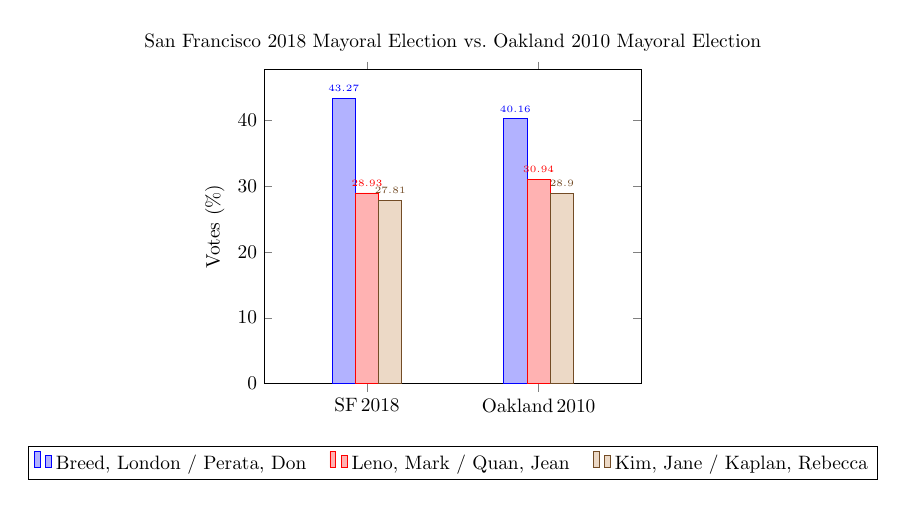
\begin{tikzpicture}[scale=0.7, transform shape]
    \begin{axis}[
      title={San Francisco 2018 Mayoral Election vs.\ Oakland 2010 Mayoral Election},
      ybar,
      bar width=12pt,
      ylabel={Votes (\%)},
      symbolic x coords={SF\,2018,Oakland\,2010},
      xtick=data,
      enlarge x limits=0.6,
      ymin=0,
      enlarge y limits={upper,value=0.1},
      nodes near coords,
      every node near coord/.append style={font=\tiny},
      legend style={
        at={(0.5,-0.20)},
        anchor=north,
        legend columns=3,
        /tikz/every even column/.append style={column sep=1em}
      },
    ] 

      \addplot+[bar shift=-12pt]
        coordinates {(SF\,2018,43.27) (Oakland\,2010,40.16)};
      \addplot+[bar shift=0pt]
        coordinates {(SF\,2018,28.93) (Oakland\,2010,30.94)};
      \addplot+[bar shift=12pt]
        coordinates {(SF\,2018,27.81) (Oakland\,2010,28.90)};

      \legend{
        {Breed, London / Perata, Don},
        {Leno, Mark / Quan, Jean},
        {Kim, Jane / Kaplan, Rebecca}
      }

    \end{axis}
  \end{tikzpicture}
  \label{fig:1}
\end{figure}

Figure \ref{fig:1} compares the vote results for three finalists in the 2018 San Francisco and 2010 Oakland mayoral election. Because the voting preference for the Oakland race in this particular round was comparable to the voting preference in the San Francisco election at the same stage, with Perata led with 40.16\%, versus Breed with 43.27\%; Quan was in second place Quan with 30.94\%, versus Leno with 28.93\%; and Kaplan was in third place with 28.9\%, versus Kim with 27.81\%. 

By Pass 9, Kaplan had in fact received more transferred votes than either Quan or Perata, gaining a 7.32\% increase from the first round, versus 6.47\% increase for Quan and 6.43\% increase for Perata. However, her initial disadvantage still put her on the elimination spot, which turned out to be crucial for Quan’s victory. Of all of Kaplan’s votes, 22.6\% were exhausted, a substantial 19.6\% transferred to Perata, but a decisive 57.7\% went to Quan, pushing her just over the 50\% threshold. 

\section{Conclusion}

Revisiting the three factors – polarization, negative and strategic campaigns, and the spoiler effect, case studies of the 2022 Alaska state Senate and U.S. Senate elections reveal that candidates who appeal to the broader population and less polarized ideas benefit in the RCV elimination rounds; case studies of the 2018 San Francisco and 2010 Oakland mayoral elections reveal that while RCV does not eliminate the presence of strategic voting and utilization of negative ads in the process, it does promotes strategic alliances between candidates, which can be advantageous in the unique RCV elimination process; case studies of 2022 Alaska gubernatorial, state House elections, and U.S. Representative prove that RCV can successfully mitigate the spoiler effect, although the center-squeeze effect potentially prevented third-place moderate candidate Nick Begich from winning the office in the special election for U.S. Representative. 

In 2022, Nevada voters passed a ballot measure to implement a “top-five primary” with open primaries regardless of voter affiliations and a RCV general election to determine the final Representative. The system will take place in the 2024 election season (\cite{clyde2022}, 2022). As RCV implementation expands through years, more observations and conclusions can be made. For example, while this paper can not definitely validate that RCV caused the bipartisan coalition in the Alaska Senate after the 2022 elections, it confirms a correlation between RCV and the incentives for candidates to appeal to bipartisan ideals (\cite{rosen2022}, 2022). As future elections proceed, researchers will have more opportunities to explore how candidate and voter behaviors evolve under RCV, leading to more definitive conclusions. 

In conclusion, this paper posits that RCV can provide tangible meaningful electoral reforms in combating polarization and the spoiler effect. While it can not definitively claim that RCV reduces negative and strategic voting, it does suggest that RCV can visibly moderate candidate behaviors, contributing to a more constructive electoral process.

\nocite{*}
\printbibliography[title={References}, heading=subbibliography]
\end{refsection}

\begin{refsection}[refs/american]

\makechapter{The American Dream's Flawed Promise of Education}{The American Dream’s Flawed Promise of Education:\\ The Issue of Academic Stress}{Charles Schäfer}{Stuyvesant High School}{10.17613/82c3s-nac44}


At the center of the American dream lies the promise of education: the idea that with hard work comes reward. Unfortunately, in such a rapidly shifting society, established standards have quickly begun to shift. The issue of academic stress and its impact on adolescents has become increasingly important in recent years. Increased competition for college and jobs has driven the academic expectations for adolescents higher and higher. High school students take more college-level classes, fill out their resumes with more extracurriculars, and score higher on standardized tests. Unfortunately, as academic demands increase, so does academic-related stress. Academic stress encompasses various stressors, such as intimidating workloads, performance pressure, and even self-inflicted stressors like time management issues. These stressors can have major long and short-term effects on one’s physical and mental health, potentially resulting in sickness for a week or even leading to long-term mental health concerns that extend into college and beyond. Despite its many detrimental effects, in the correct environment, academic stress can be turned into resilience and strength. The importance of the impact of academic stress is creating educational institutions that support students’ personal growth, rather than enforce detrimental stress. Addressing this issue is vital for improving students' academic performance, well-being, and future. While academic stress can have severe short-term consequences and devastating long-term effects, supportive educational environments can alleviate stress and promote resilience. 

Excessive academic stress in challenging environments can cause significant short-term repercussions, including anxiety and depression, feelings of inadequacy, and even physical consequences. Periods of peak stress in academically rigorous environments, particularly distance learning, correlate with increased depression and anxiety. In academically stressful environments, students are typically juggling tests, homework, and high grades. This balancing act puts extreme strain on the overworked student: “Sudden bursts of academic stress significantly undermine emotional health and well-being” (\cite{claney2023}). In addition, stressful environments heavily contribute to increasing stress and its repercussions. One of the most stressful environments for students was the COVID-19 pandemic, where distance learning saw increased depression among college students due to feelings of isolation and academic pressure (\cite{chen2024}). Locked in their rooms for the majority of the day, academic stress only amplified growing feelings of depression. Unfortunately, academic stress during the pandemic was pervasive, with 90 million cases of anxiety and 70 million cases of depression being newly measured (\cite{cordovaolivera2023}). According to a study conducted on 1200+ university students, 35\% reported having experienced depression from academic stress during the pandemic (\cite{cordovaolivera2023}). While stressful environments and moments of maximum stress can cause severe depression and anxiety, many other stressors can cause different psychological challenges. Self-imposed stressors, such as time management and perfectionism, exacerbate feelings of inadequacy and emotional instability. Self-imposed stressors are traits people have that often cause feelings of insecurity. Typically, these stressors are based on students' subjective beliefs about their ability to meet their academic goals, creating continuous pressure and a sense of failure if one’s high expectations are unmet (\cite{cordovaolivera2023}). The most common stressor, poor time management, was identified as the “most significant stressor for university students, leading to feelings of emotional instability” (\cite{cordovaolivera2023}). Other self-imposed stressors, such as maladaptive perfectionism or “hypercritical judgment upon failure to meet extreme goals”, are also associated with negative self-perception (\cite{almroth2019}). These toxic forms of introspection can reinforce feelings of inadequacy, whereas fear of failure can hinder one’s ability to confidently approach schoolwork and life as a whole. Research from the National Longitudinal Survey of Adolescent Health reveals that self-perception of inadequacy contributes heavily to emotional instability and fear of failure (\cite{mcleod2012}). This feedback loop of self-inflicted stressors increasing negative self-perception and emotional instability is exceedingly unhealthy, often manifesting itself in physical effects. Prolonged stress results in physical consequences including sleeplessness, changes in appetite, and a weakened immune system. One of the most common physical effects of stress is sleeplessness. This is caused when acute stress attacks increase heart rate and dilate blood vessels to direct blood to large muscles and the heart, elevating blood pressure in a "fight or flight" response (\cite{sha2023}). These attacks come unpredictably, resulting in sleeplessness as the body attempts to return to normal. Unfortunately, once stressed individuals are asleep, they experience “sleep disturbances”, where stress activates neurons in the hippocampus region causing interruptions or low-quality sleep (\cite{mcleod2012}). Another physical consequence of stress is an altered appetite, causing an increase or decrease in food intake, resulting in unhealthy eating patterns and weight fluctuations (\cite{sha2023}). Finally, extreme stress can lead to prolonged cortisol release, weakening the immune system and making the body more susceptible to illness (\cite{cordovaolivera2023}). While periods of extreme stress can have many short-term repercussions, long-term exposure to stress can have devastating permanent effects.

Chronic academic stress can have the long-term negative effects of creating poor stress management habits, increasing the chances of long-term physical weakness, and fostering permanent emotional and psychological damage. Unresolved stress from a high academic workload in adolescence weakens one’s ability to manage future stressors, leading to unhealthy coping strategies in adulthood. Adolescents under constant academic pressure are less likely to develop effective coping mechanisms, as stress often overrides cognitive strategies for stress management (\cite{chen2024}). Lowered self-worth caused by chronic academic stress can cause individuals to perceive future stressors as insurmountable. Over time, this causes students to develop maladaptive coping mechanisms or self-destructive methods for treating stress (\cite{cordovaolivera2023}). Repeated stress responses during the formative years of adolescence can influence how people respond to such stress in adulthood. Such stress-resolving strategies that carry over from adolescence can include “avoidance, denial, or substance abuse” (\cite{claney2023}). This can have massive effects on one’s professional and personal life, disrupting one’s career and relationships. In addition, extreme bursts of academic stress can activate the HPA axis, an anti-stress bodily system that causes sustained cortisol release (\cite{cordovaolivera2023}). This can impair cognitive and emotional regulation, making future responses to stress extremely ineffective. Similar to stress-coping habits, repeated physiological responses also cause permanent bodily harm. Persistent academic stress can permanently increase cardiovascular, immune, and cognitive weakness. Maintaining cardiovascular health is extremely important in living a healthy life. Unfortunately, long-term stress contributes to persistent increases in heart rate and blood pressure, which elevate the risk of hypertension, heart attack, and even stroke. Chronic stress also creates inflammation in coronary arteries, increasing the risk of cardiovascular disease (\cite{almroth2019}). All of these cardiovascular repercussions are associated with long-term chronic stress. Unfortunately, chronic stress can also damage other parts of the body: chronic stress also impairs communication between the immune system and the aforementioned HPA axis, leading to increased vulnerability to “chronic fatigue, metabolic disorders (e.g., diabetes, obesity), and immune dysfunction” (\cite{sha2023}). Beyond weakened cardiovascular and immune systems, academic stress can severely damage an adolescent’s cognitive abilities. Similar to trauma, chronic stress can negatively impact memory, attention, and cognitive function–all essential for learning and development. Stress also makes individuals more susceptible to mental health disorders like PTSD, Major Depressive Disorder, and Bipolar Disorder (\cite{claney2023}). Yet another burden that stress can have on the body is also seen in the continuous activation of the autonomic nervous system and immune system which can lead to long-term wear-and-tear on the body, causing exhaustion and a weakened physical state (\cite{almroth2019}). It is imperative to recognize stress’s wide-reaching consequences on the body, and how such a small part of one’s life can have devastating effects. Beyond physiological consequences, academic stress can also have deeper ramifications by affecting one’s attitude and drive. Excessive academic stress during adolescence increases the likelihood of persistent emotional and psychological challenges into adulthood including lessened motivation, reduced self-esteem, and reliance on external validation. Repeated academic stress can be extremely demoralizing, sapping the determination that one may have had prior. Chronic academic stress during adolescence is linked to long-term emotional exhaustion, reduced motivation, and an increased likelihood of burnout (\cite{cordovaolivera2023}). Extreme stress often causes academic or workplace struggle; repeated failure is not only demoralizing but also detrimental to one’s outlook on life. This is seen when people underestimate their abilities, perceiving themselves as weaker than their aspirations. Long-term academic stress correlates with an increased risk of self-esteem issues and psychological distress later in life (\cite{almroth2019}). With lowered self-esteem in adolescence, those with chronic stress often foster a dependency on external validation for self-worth (\cite{cordovaolivera2023}). In contexts where academic success is heavily emphasized, students frequently equate their value with external achievements and validation (\cite{almroth2019}). Arbitrary statistics such as GPA and test scores can massively impact a student’s mental health. If unresolved, this trend will continue into adulthood, where individuals struggle with identity and self-worth in a more consequential environment. Academic stress has many extremely negative long and short-term consequences on the body and mind; luckily, academic stress, in tandem with rigorous support, can benefit and strengthen adolescents. 

The extreme consequences of academic stress can be alleviated through rigorous support in providing stress-abating resources, promoting strong feelings of school belonging, and fostering resilience to transform stress into growth. Supportive academic environments provide stress-relieving resources and services such as crisis hotlines and mental health centers. With academic stress being so prevalent among students during the pandemic, many high schools and universities integrated crisis hotlines into their mental health resources. 
Institutions such as Wake Forest University promote hotlines such as The Oregon YouthLine, The Trevor Project, and the National Suicide Prevention Lifeline (\cite{wfu2025}). These hotlines, typically open continuously, provide service to those requiring immediate assistance or those simply needing someone to talk to. Such hotlines are extremely effective, with a 2020 study finding a 43\% decrease in overall caller distress, and a 56\% caller follow-up rate (\cite{boness2021}). Other stress-relieving resources have also found great success in supporting student mental health. Following the pandemic, the National Association of Student Personnel Administrators (NASPA) published research regarding strategies for helping students facing academic stress, citing on-campus counseling and support groups as the most effective methods to counteract academic stress (\cite{wfu2025}). School-provided support groups are beneficial due to their communal element. Interacting with students in similar situations promotes connection associated with “enhanced well-being and reduced stress” (\cite{duan2016}). Beyond school-based mental health centers, academically stressful environments can also alleviate stress by promoting a culture of school connectedness. A strong sense of school belonging correlates with lower symptoms of depression and anxiety, promoting resilience to stress. With lowered self-esteem being a major symptom of academic stress, feeling socially valued in one’s community can combat these negative feelings. This feeling of acceptance can largely reduce anxiety and depression symptoms in adolescents, seeing a marked drop after 12-18 months (\cite{allen2024}). Even long-term effects of chronic stress, including predisposition to mental health disorders, can be mitigated through feelings of school belonging. In a longitudinal study conducted on Australian high school and college students, those studying in socially welcoming environments saw a gradual decline in mental health symptoms over time, whereas those studying in purely stressful environments saw sharp increases in depression and anxiety (\cite{allen2024}). Social factors play a major role in influencing how adolescents approach schoolwork and stress. If supported by one’s peers, students are often pushed to work harder to compete with their peers. This can result in increased academic engagement and, by extension, resilience to stress. A 2022 study conducted on Dutch university students determined that engagement was a key pathway to resilience, with 78\% of engaged students reporting resilience to stress (\cite{versteeg2022}). Supportive environments prevent academic stress from hindering their students and transform experienced stress into strength. Supportive school environments cultivate mental resilience, stress-mitigating skills, and strength. Resilience plays a major role in turning stress into strength. Defined as the “ability to bounce back from adversity”, resilience is critical for adolescents in academically challenging environments (\cite{claney2023}). Supportive academic environments utilize stress management activities that promote resilience, such as mindfulness and physical activity. Mindfulness, the practice of “focusing on the present moment non-judgmentally”, fosters relaxation and a sense of calm (\cite{claney2023}). This can help teens cope with the pressures of school by disconnecting from external stressors to reduce anxiety. Physical activity can similarly act as a stress reliever: producing endorphins to improve mood, allowing the individual to detach themselves from their problems, and improving bodily health. In a study conducted by the American Psychological Association, 62\% of adults reported physical activity as “extremely effective” in reducing stress (\cite{apa2014stress}). These stress-relieving techniques can increase one’s resilience to stress, allowing their experience to grow into strength. By fostering resilience through mindfulness and physical activity, schools help students manage stress to build strength. With the correct support, stress becomes a tool for growth rather than a burden, fostering a healthy mindset and academic success. 

The American Dream has long been the golden standard that all strive for. Traditionally, the dream was defined as the promise that hard work is rewarded by material wealth and other classic markers of success: owning a house with a white picket fence, going to a good college, and living patriotically. These dreams have brought millions of immigrants to America and motivated countless generations. As our society’s standards and goals change, the American Dream for many has shifted to incorporate new aspirations, often centered around personal freedom: being financially independent, finding meaningful relationships, and, most importantly, being healthy, happy, and emotionally fulfilled. For adolescents, traditional American values prioritizing strong education can take precedence over core human values of being healthy and fulfilled. Chronic academic stress can force a reliance on external validation from markers like GPA and test scores. Luckily, the shift from traditional American values to more relevant human ones promotes support for academic stress and a greater focus on the more important aspects of life: happiness, health, and fulfillment.



\nocite{*}
\printbibliography[title=References,
heading=subbibliography]
\end{refsection}

\begin{refsection}[refs/moralint]

\makechapter{Against Moral Intuitionism}{Against Moral Intuitionism}{Celine Wang}{Farmington High School}

\section{Introduction}

In this paper, I contend that we do not have any reason to trust in our moral intuitions on the grounds that moral intuitions are epistemically unreliable, suffer from persistent disagreement, and are subject to debate regarding its objectivity. 

To limit the scope of our discussion, I will be focusing on a foundationalist interpretation of intuition as a means of knowledge production (\cite{britannica2024intuition}). As such, an intuition shall thereby be defined as a self-evident “intellectual seeming” (\cites{audi1999self}[p.\ 10]{bealer1998intuition}[p.\ 102]{huemer2005ethical}[p.\ 1]{ogar2016critique}). Consequently, moral intuitionism would entail a non-natural, realist stance on the objectivity of morality, and would be the utilization of intuition as an epistemic tool concerning moral matters; i.e., what is right and what is wrong (\cites{ethics2024moral}{stratton2014intuitionism}).  

\section{Argument From Unreliability}

As opposed to perception, intuition is notoriously unreliable. While not infallible, perceptual seemings (i.e., the visual analog of intellectual seemings) are typically considered reliable because they detect potential inaccuracies \emph{vis-à-vis} context. In other words, when weather phenomena obscures vision or when physically impaired, we are less apt to trust our perceptual seemings (\cite[p.\ 8]{cecchini2024reliability}). Intellectual seemings, on the other hand, lack the capacity to receive reliable feedback contextually (\cite[pp.\ 17–18]{destefano2014reliability}).

Additionally, the non-naturalness of moral intuition implies that they are causally inert, i.e., they can neither affect nor be affected by other objects. That is to say, moral intuitions cannot be caused by their corresponding moral truths (\cites[p.\ 1]{hayward2019immoral}{stratton2014intuitionism}).

Moral intuitions are also subject to various distorting factors.  

First, phraseology. Studies have concluded that when the trolley problem was presented with “saving language”, people overwhelmingly choose to flip the switch; the opposite occurred when “killing language” was employed (\cite[p.\ 6]{bengson2013experimental}).

Second, partiality. One might have ulterior motives for experiencing certain intuitions (\cite[pp.\ 343–346]{sinnott2006moral}). For example, in judging two piano performances, the father of one of the contestants would, intuitively, think that his daughter played better, though this might not be justified without familial association (\cite[p.\ 343]{sinnott2006moral}).

Third, disgust. Disgust elicited by physical or chemical stimuli and disgust regarding some moral prospects, respectively, have been shown to influence the moral intuitive process (\cite[p.\ 8]{tao2022effects}).

Moreover, other factors also influence intuition. These include the ordering of cases involving intuition, hunger level of intuitive moral agents, and the “Knobe effect,” i.e., the tendency for people to judge intentional actions as negative rather than positive (\cites{swain2008instability}[p.\ 1]{danziger2011extraneous}).

An argument which has been proposed by Jonathan Smith states that partiality is imprecise. Concerning the example mentioned previously, Smith argues that a piano performance is incomparable with moral intuition. There are nuances and particularities present in musical performances which are not present in the fundamental claims of basic moral intuitions (e.g., murder is bad). He presents a counterexample: two contestants play a single note and are judged based on proximity with a third note. Thereby, if the father judges that the note his daughters played was closer, then he would be justified in believing that his daughter won, regardless of his familial predisposition towards her (\cite[p.\ 77]{smith2010sinnott}).

Though I agree that the father would be justified in the second instance, this argument assumes a moral realist conclusion. A better reformulation of the piano competition would be one in which the two contestants are simply told to simply play one note. The father is then asked simply, “Who played better?” By eliminating the intended note (or, when applied to the topic of moral intuitionism, some accepted moral principle), partiality comes back into play. 

Considering another possibility, Dario Cecchini suggests that the strength of intuition may be a method of tracking the potential reliability of intuition in a context-sensitive way. This would only be the case if one truly accepts moral intuitions proportional to confidence in said intuitions, and that such confidence is epistemically reliable (\cite[p.\ 11]{cecchini2024reliability}). One’s confidence would then accordingly be used to determine the presence of biases, and as such, eliminating the possibility of distorted intuitions. 

Nonetheless, there are inconsistencies in this argument. The idea that intuitive strength is epistemically reliable remains hotly contested, as it currently lacks sufficient empirical study (\cite[p.\ 22]{cecchini2024reliability}). Furthermore, it seems unlikely that one would be able to prove the epistemic reliability of moral intuitions, given that intuitive strength itself is subject to distorting factors such as the Dunning-Kruger effect or the “consensuality principle” (\cites[pp.\ 23–24]{cecchini2024reliability}[pp.\ 259–262]{dunning2011kruger}{koriat2012self}). Such an argument is also subject to the implication that self-evidence is strength dependent, which undermines the very definition of the term itself. 

\section{Argument from Disagreement}

One might assume that since moral intuition is “self-evident” and “non-inferential,” that there would be harmony between proponents of moral ideas. Yet, this is not the case. When ten diverse societies were examined for their views regarding moral principles, each “exhibited substantial variation not only in the degree to which such [moral] factors were viewed as excusing, but also in the kinds of [moral] factors taken to provide exculpatory excuses, and in the types of norm violations for which such [moral] factors were seen as relevant” (\cite[p.\ 4692]{barrett2016small}). If the moral intuitions of two unprejudiced individuals persistently disagree on some moral issue, then the realist basis for intuitionism would be compromised (\cites[pp.\ 208–210]{sidgwick1907methods}[p.\ 44]{shaferlandau2004good}).

In addition, what seems “moral” to us may be evolutionarily favored biological responses that have emerged over time. We have evolved to react to different moral acts with either approval or disapproval based on biological necessity, preventing us from attaining positive knowledge of moral predicates (\cites[p.\ 348]{singer2009ethics}[p.\ 72]{joyce2007evolution}{morton2016new}). Differences in moral beliefs have also been observed across ages and between modern and traditional culture groups (\cite{nisan1987moral}). One especially notable example of moral disagreement is the disagreement between moral collectivists and individualists, as many common moral realist objections directed towards the idea that their disagreements will not remain persistent, have been disproven (\cite[pp.\ 855–864]{goldman2022right}).

Nevertheless, this is a shallow argument, as non-moral disagreements are not the true point of contention in a moral issue. In comparison with the previous example, we would certainly object if a living person were to be boiled, even without experiencing pain. The question again returns to a moral one: Are the lives of a lobster and a person worth the same? If one continues to argue that “worth” could be determined via some empirical measure, e.g., brain capacity, then a new moral issue emerges: is it morally acceptable to boil some organism simply based on the metric of brain capacity? This line of argument suggests the infinite regressive loop fallacy.  

Russ Shafer-Landau proposes that the argument from moral disagreement is self-defeating. He summarizes said argument in terms of moral realism, a key property of intuitionism: 
\begin{enumerate}
	\item[P1:] \textit{Moral realism is subject to persistent disagreement;}

	\item[P2:] \textit{Any theory(s) subject to persistent disagreement is false;}

	\item[C:] \textit{Therefore, moral realism is false (\cite[pp.\ 44–48]{shaferlandau2004good})}.
\end{enumerate}

To this, he claims that the same argument could be applied in reverse. Substituting “moral realism” for “theories against moral realism” results in the conclusion that theories against moral realism are false. 

As we will see, though Shafer-Landau’s argument is valid, it is not sound. Concealed by Shafer-Landau’s summary of the argument from disagreement is what I will term the agreement premise. The premise states that if moral realism is true, then there would be widespread agreement regarding moral realism. 

\begin{enumerate}

	\item[P1:] \textit{The agreement premiss is true;}

	\item[P2:] \textit{Moral realism is subject to persistent disagreement;}

	\item[P3:] \textit{Any theory(s) subject to persistent disagreement is false;}

	\item[C:] \textit{Therefore, either (a) moral intuitionism is false, or (b) the agreement premise is false.}

\end{enumerate}

Accepting either (a) or (b) would be difficult for the moral realist. Conversely, if one were to now substitute “moral realism” for “theories against moral realism,” then (b) would be acceptable to opponents of moral realism, as it implies that only some would agree with moral realism, perfectly. In other words, Shafer-Landau’s argument, though compelling, is more so \emph{vis-à-vis} the moral realist. 

\section{Argument from Queerness}

Moral Intuitionism is a theory that is built upon a foundation of self-evident, non-inferential moral objectivity. However, the very existence of such values can be challenged. In J. L. Mackie’s Argument from Queerness, Mackie reasons such that if objective values were to exist, then objectively good values would have an inherent “to-be-pursuedness,” and objectively bad values would have an inherent “not-to-be-pursuedness” (\cites[p.\ 40]{mackie1978ethics}[p.\ 104]{olson2014moral}). This motivational property is one that is unique to objective moral values, and one which cannot be described in naturalistic terms; in other words, objective values are “queer” (\cites[pp.\ 2–3]{scholl2015defense}[p.\ 33]{mackie1978ethics}) To claim that such a property is not queer is to invite contradiction with the non-natural property of moral intuitions (\cite[p.\ 41]{mackie1978ethics}). The argument can be represented in both metaphysical and epistemological versions, however, only the epistemological is necessary here:  

\begin{enumerate}

	\item[P1:] \textit{If objective moral values exist, they will have to be epistemologically queer, and require unconventional, bizarre epistemological faculties;}

	\item[P2:] \textit{We are unable to utilize such bizarre epistemological faculties;}

	\item[C:] \textit{We should not believe that objective moral values exist (\cites[pp.\ 38–41]{mackie1978ethics}[pp.\ 1–2]{lillehammer2019queerness}).}

\end{enumerate}

The parity argument, proposed by Terence Cuneo, attempts to prove the existence of objective values. His argument has two main premises: the parity premise ($P_P$) and the epistemological realism premise ($P_E$). The parity premise states that moral facts and epistemic facts are analogous to one another since both are categorical imperatives, i.e., both tell us what we ought to do and believe regardless of our subjective desires. The epistemic realism premise describes the idea that belief in the existence of epistemic facts seems natural; otherwise, one could theoretically have misconstrued beliefs based only on whims and compulsions (\cite[pp.\ 52–62]{cuneo2010normative}). His argument is outlined as the following, with an extra “modus tollens” ($P_{MT}$) premise added for clarity:
\begin{enumerate}

	\item[P1:] \textit{If objective moral values exist, they will have to be epistemologically queer, and require unconventional, bizarre epistemological faculties;}

	\item[P2:] \textit{We are unable to utilize such bizarre epistemological faculties;}

	\item[C:] \textit{We should not believe that objective moral values exist (\cites[pp.\ 38–41]{mackie1978ethics}[pp.\ 1–2]{lillehammer2019queerness}).}

\end{enumerate}

The parity argument, proposed by Terence Cuneo, attempts to prove the existence of objective values. His argument has two main premises: the parity premise ($P_P$) and the epistemological realism premise ($P_E$). The parity premise states that moral facts and epistemic facts are analogous to one another since both are categorical imperatives, i.e., both tell us what we ought to do and believe regardless of our subjective desires. The epistemic realism premise describes the idea that belief in the existence of epistemic facts seems natural; otherwise, one could theoretically have misconstrued beliefs based only on whims and compulsions (\cite[pp.\ 52–62]{cuneo2010normative}). His argument is outlined as the following, with an extra “modus tollens” ($P_{MT}$) premise added for clarity: 
\begin{enumerate}

\item[$P_P:$] \textit{There can be no epistemic facts if there are no moral facts;}

\item[$P_E$:] \textit{There are epistemic facts;}

\item[$P_{MT}$:] \textit{If there are epistemic facts, then there are moral facts;}

\item[C:] \textit{If there are moral facts, then moral realism is true (\cite[p.\ 1]{rutten2010parity}).}

\end{enumerate}

Believing in moral realism, by definition, entails believing in objective moral values, and in this case, moral intuitionism. 

Regardless, though the argument is valid, the parity premise lacks argumentative power. As Richard Joyce notes, there are many ways in which moral facts and epistemic facts are incompatible. Examples include how unlike with moral facts: 

\begin{enumerate}

	\item We acquire epistemic facts involuntarily.

	\item Epsitemological facts lack the concept of desert, i.e., "deserved reward or punishment (\cite{merriam2024desert})."

	\item We are not reluctant to rely on the judgement of experts when faced with epistemological facts (\cite[pp.\ 14–16]{joyce2007evolution}).

\end{enumerate}

As a result of these discrepancies, we can safely disregard the parity argument and regard the argument unsound.  

Hallvard Lillehammer expresses another objection, claiming that knowledge of objective moral values does not entail the utilization of epistemologically queer faculties (\cite{balaguer2016platonism}). He argues that moral facts can be equated with logical facts, since both are causally inert (\cite{balaguer2016platonism}). Hence, as Lillehammer points out, if logical facts rely only on an “unproblematic sense … which we are able to grasp” and not some bizarre epistemological faculty, then the same should be the case for moral facts. If one were to deny this argument, the implication would be that we are unable to access logical facts, a highly contentious and counterintuitive claim (\cite[p.\ 6]{lillehammer2019queerness}). 

Whilst claiming that logical facts are epistemologically inaccessible is certainly absurd, we can nonetheless dispute the notion that logical facts and moral facts are analogous. One key disanalogy between the two lies in that logical facts lack the “to-be-pursuedness” of moral facts. For example, while the moral fact “giving to charity is good” carries an inherent tendency to act, a tautology such as “all humans are mammals” does not (\cite{britannica2024tautology}). 

\section{Conclusion}

I have presented three arguments against moral intuitionism in this paper, including how:

\begin{enumerate}
\item Moral intuitions are fallible.

\item There are disagreements between supposedly ``self-evident'' moral intuitions.

\item The objective nature of moral intuitions can be challenged.
\end{enumerate}

Thus, I reject the notion that we have any good reason to trust our moral intuition.


\nocite{*}
\printbibliography[title=References, heading=subbibliography]
\end{refsection}

\begin{refsection}[refs/farm]
\makechapter{The Political Economy of Farm Subsidies}{The Political Economy of Farm Subsidies}{Sarah Kim}{Las Lomas High School}{10.17613/82c3s-nac44}

“America, land of the free”—or so they say. In reality, the United States is far from being a genuinely free nation. The American government has a well-documented history of abusing its considerable power, including in the protection of slavery, restriction of voting rights, and suppression of dissent. However, what is less well-known but hugely significant is the government’s intervention in agriculture. The roots of this extensive involvement lie in the Agricultural Adjustment Act of 1933, which was enacted to stabilize farm prices during the Great Depression. Decades after the Depression, however, the government has continued to subsidize agriculture. Furthermore, while aimed at aiding farmers and lowering prices, government intervention has been highly detrimental, impacting both the U.S. and the international community. In essence, the American government’s agricultural intervention exemplifies the coercive nature of government and underscores the need to limit such practices in society.  

Although the original intention of subsidies was to alleviate the plight of struggling farmers during the Great Depression, farmers are no longer in the same desperate straits. They are thriving, in fact. Paradoxically, despite farmers’ average incomes being 52 percent above the national average and their net worth reaching eight times the average American’s net worth, the government continues to subsidize their income. Indeed, nearly 40 percent of farmers’ income is derived from government aid. Furthermore, subsidies are regressive in nature. In 2019, only around 3 percent of American farmers collected nearly 70 percent of subsidies; on average, from 1995 to 2021, while the bottom 80 percent of farmers received around 9 percent of all federal allocations, the top decile received nearly 78 percent of the total. Since many farm subsidies are distributed based on a certain farm’s historical production volume, and larger farms have higher production volumes, they are given the majority of federal subsidies. Additionally, there is the problem of subsidy-induced overproduction, which leads to artificially suppressed food prices. However, to maintain prices, the government has set price floors for various farm products. The sugar price floor, for instance, results in an annual cost of approximately \$4 billion for consumers. Beyond this, consumers also face a tax burden of roughly \$206 per household per year to finance the government subsidy programs. It is also ironic that the government, after creating a supply glut through subsidies, then purchases and resells excess goods internationally at a steep discount. In this way, the government incurs significant financial losses, effectively subsidizing foreign consumers at the expense of U.S. taxpayers. As evidenced, farm subsidies produce inequality, long-term market distortions, and increased costs for consumers, compromising the overall health of the U.S. economy. 

Beyond these domestic repercussions, the impact of American farm subsidies is felt worldwide. Typically, developing countries have a comparative advantage in producing agricultural goods. However, this advantage is nullified by the subsidization of products produced by more developed nations. The ramifications of this are substantial for developing economies. Each year, such subsidies cost developing nations around US \$24 billion, not accounting for any spillover effects; the inclusion of such effects would yield a significantly higher total, given that agriculture often comprises a large portion of developing nations’ economies. Studies have shown that a 1 percent increase in Africa’s total agricultural exports would lift its GDP by US \$70 billion per year, roughly five times the amount of foreign aid received in the same period. Clearly, even beyond the U.S., farm subsidies have had devastating effects. 

Having illustrated the failings of subsidies, we should naturally ask ourselves, \emph{why do they still exist?}  The answer to this question lies in politics. Just like any other government program, the recipients of aid create interest groups that fiercely defend their handouts, relentlessly perpetuating the myth of the struggling family farmer whose woes require overwhelming federal subsidies to remedy. Nonetheless, such is a narrative detached from reality. Another method of maintaining farm subsidies is by aligning them with food security, that is, presenting a bill to Congress that includes both farm subsidies and food security proposals. By linking farm subsidies to food security, opposition to subsidy programs is framed as an assault on the food-insecure, transforming a discussion of economic policy into a morally condemnatory criticism of political opponents.  

In summary, farm subsidies exemplify government coercion in two primary ways. First, farm subsidies erode public trust in the government by fostering an environment in which politically connected agricultural interests benefit at the expense of both domestic consumers and vulnerable populations abroad. Second, farm subsidies undermine the individual freedom of farmers and consumers. Consumers are unwittingly coerced into funding the livelihoods of wealthy farmers, while smaller farmers struggle to survive under government-imposed disadvantages. Overall, farm subsidies represent a clear example of government overreach. Where the free market would have been able to allocate resources efficiently, the government has stepped in to forcefully disrupt the equilibrium. 

When the government is unchecked in its power, it no longer acts with the interests of the people in mind, leading to policies that demand compliance rather than reflect consent. In addition, the government is unable to adapt to changing circumstances. What was once a measure intended to buttress the agrarian base of the U.S. economy has now become a means of entrenching wealth inequality. Although government intervention can have benevolent intentions, it usually erodes individual liberty, distorts the free market, and often reverses the intended effects of wealth redistribution, with taxpayers coerced to fund the endeavor. Ultimately, it is vital to uphold the principle of limited government, ensuring that policies do not become the means by which the state undermines the foundations of a free society. As economist Henry George once observed, “Government should be repressive no further than is necessary to secure liberty… and the moment governmental prohibitions extend beyond this line they are in danger of defeating the very ends they are intended to serve.” It is imperative that the government’s function be that of an impartial umpire, rather than an active stakeholder. Markets, not governments, create prosperity. 


\nocite{*}
\printbibliography[title=References,heading=subbibliography]
\end{refsection}

\begin{refsection}[refs/asymmetry]
\makechapter{The Asymmetry of Moral Obligations}{The Asymmetry of Moral Obligligation}{Sam Cao}{Miramonte High School}{10.17613/x9f1v-kk381}{10.17613/n9xdf-8dh92}

\section{Introduction}

This paper examines our moral obligations to current and future generations, as well as the accompanying policy implications. Although many analyses attempt to resolve the problem by outlining specific moral obligations, I argue that such an approach is ineffective. Moral disagreement pervades today’s cosmopolitan societies, demanding that we address such disagreements pragmatically. Thus, a deeper question emerges: How can we manage division regarding moral obligations? Regarding this concern, I contend that while we might ground obligations to the living primarily in traditional morality, obligations to future people would depend exclusively on instrumental reasoning.

\section{Justifying a Meta-Ethical Approach}

Putatively, a moral obligation is defined as a demand that an agent ought to fulfill, such that failing to do so constitutes wrongdoing (\cite{pick2004} pp.\ 26–27).

Although this definition implies that moral obligations are broadly recognized, this is farfrom the truth; agents frequently contest even fundamental principles such as justice, fairness,and impartiality (\cite{atari2020}). Many national and international concerns, such as climate change, resource overconsumption, and national debt, expose deep moral disagreements (\cite{hasan2023}). This paper specifically
focuses on climate change. Faced with the issue of greenhouse gas emissions, developed and
developing nations offer contradictory judgments: developed economies advocate for universal emissions reduction requirements, asserting that climate change cannot be contained if any parties are exempt, whereas developing nations assign such burdens exclusively to developed nations, citing universal emissions cuts as unjust barriers to industrialization (\cite{belfiori2024}). Due to the absence of a common moral foundation, one’s view of morality may seem arbitrary or even repugnant to others. Additionally, we do not know how future values might differ from contemporary values,
undermining the relevance of fixed moral rules grounded in the former (\cite{macaskill2019}). Thus, a universally agreed-upon understanding of moral obligation cannot exist.

The priority then shifts from laying down fixed moral precepts to fostering cooperation both among current agents and between current and future agents.\footnote{For varied arguments against a prescriptivist view of morality, see Francesco Allegri, \emph{Conflicting Values and Moral Pluralism in Normative Ethics}; David B. Wong, \emph{Natural Moralities: A Defense of Pluralistic Relativism}; and Jonathan Dancy, \emph{Ethics Without Principles}.} Contractarianism, a subset of social contract theory, suits this approach. Beyond its grounding in mutual benefit and respect for individual autonomy present in all social contract theories, it also features a motivationally internalist structure and requires only that agents possess basic instrumental rationality.\footnote{For more general arguments vis-à-vis a moral social contract approach, see Jan Narveson, \emph{Social Contract: The Last Word in Moral Theories}; Kelly James Clark, \emph{Why Be Moral? Social Contract Theory Versus Kantian-Christian Morality}; Susan Dimock, \emph{Two Vritues of Contractarianism}; Rucha Kulkarni, \emph{A Critical Analysis of Moral Contractarianism: Towards a Revised Framework}.} Despite these advantages, traditional contractarianism confronts three key challenges: establishing trust among agents in the absence of preexisting norms (the assurance problem); maintaining compliance among self-interested agents (the compliance problem); and grounding moral agreements in non-moral reasons (the “wrong kinds of reasons” objection, which argues that actions motivated by non-moral considerations generate no genuine moral duty) (\cites[pp.\ 3–4]{kogelmann2019}[pp.\ 347]{sayremccord2013}[pp.\ 15–16]{moehler2020contractarianism}{prichard1912}). To address these concerns, this paper adopts a further evolution of contractarianism: Michael Moehler’s \emph{multilevel social contract theory.}

\section{Minimal Morality}
\label{sec:minimal_morality}

Multilevel social contract theory introduces a bifurcation of morality into \emph{first} and \emph{second}-\emph{level} morality. First-level morality, also known as traditional morality, arises from informal, often intuitive norms shaped by the existing conditions of a society. First-level morality rests on two assumptions: first, that agents possess commitment power, whereby established norms are upheld even when defection offers short-term gain; and second, that agents are not bound by prescriptive beliefs, whereby norms already shared are maintained (\cites[pp.\ 5–6]{moehler2020contractarianism}[p.\ 229]{moehler2024diversity}). One way to capture this level is through David Hume’s moral conventionalism, which holds that although agents are self-interested, they are also “morally sensible,” adhering to the two assumptions outlined above (\cites{hume1998}[pp.\ 232-233]{moehler2024diversity}). In effect, first-level morality offers a putative account of moral norms.

In contrast, second-level morality relies on self-interested bargaining conducted by rational agents, whom Moehler refers to as \emph{homo prudens}. These agents:
\begin{enumerate}

\item value long-term cooperative gains, and

\item base decisions on instrumental rationality and empirical assumptions regarding social cooperation (\cites[p.\ 8, 48]{moehler2020contractarianism}[p.\ 234]{moehler2024diversity}).

\end{enumerate}
From (i) and (ii), \emph{homo prudens} derive the weak principle of universalization (WPU), a key bargaining constraint that guides action in second-order morality (\cite[pp.\ 48–52]{moehler2020contractarianism}). According to the WPU, agents act upon the likely outcomes of hypothetical negotiations, treating others according to their basic needs and beyond that threshold, according to their relative hypothetical bargaining power (\cite[p.\ 50]{moehler2020contractarianism}). As such, the WPU both facilitates stable cooperation on the basis of non-moral values
and ensures the survival of its contracting agents (\cite[p. 50]{moehler2020contractarianism}).

A crucial structural element of multilevel social contract theory is that, as long as agents share the non-moral goal of long-term peaceful cooperation, moral contracts can be formulated to address increasingly localized disagreements (\cite[p.\ 54]{moehler2020contractarianism}). In other words, \emph{n}th levels of morality can emerge beyond second-level morality, all based on hypothetical bargaining premised on the WPU. These successive layers of moral contracts follow the principle of subsidiarity: problems should be addressed at the most local level (\cite{merriamwebster2025}). In practice, this means that agents defer to higher-level morality only when there is moral disagreement at a lower level (\cite[p.\ 235]{moehler2024diversity}). As an \emph{ultima ratio}, agents who break the contract are excluded entirely (\cite[p.\ 58]{moehler2020contractarianism}). The successive layers of morality effectively ensure the resolution of moral conflicts without compromising the overarching cooperative framework.

In addition, these moral layers supply substantive solutions to traditional contractarianism’s objections. First, the assurance problem is resolved through first-level morality, which presupposes existing moral norms, thereby bypassing the need to cultivate trust among agents who lack prior moral consensus. Second, the compliance problem is addressed by the principle of subsidiarity, as aligning moral rules closely with prudential interests deters agents from defecting. Third, the “wrong kinds of reasons” objection is mitigated by recognizing that second-level morality is not meant to replicate first-level norms; rather, we should in fact expect a divergence in the way morality is justified, as agents invoke second-level morality only when first-level morality proves insufficient.

Finally, a further concern often raised about a multilevel approach is the potential for entrenched power asymmetries: if power differentials expand to such a degree that those in power can be certain that they will remain powerful, such agents will not act in accordance with the WPU. To address this, Moehler proposes the \emph{veil of uncertainty}, arguing that even powerful agents act prudently as shifts in power differentials are unpredictable (\cite[p.\ 144]{moehler2018minimal}). However, as Brian Kogelmann notes, cases such as the Greek and American Constitutions challenge the idea that power asymmetries can be neutralized by uncertainty: these constitutions illustrate the writers’ favoritism toward their own, particularly economic, interests (\cite[p.\ 5–6]{kogelmann2019}) That being said, at its core, the objection regarding the framers of constitutions acting in self-interest misrepresents what bargaining under the WPU entails. Although this may conflict with first-level moral sensibilities, agents favoring their own interests are a predictable feature of second-level morality. Furthermore, although power disparities may favor the framers, these constitutions still safeguard every stakeholder’s basic needs; hence, they remain consistent with the WPU and second-level morality.\footnote{Both the Greek and American constitutions explicitly outline protections for basic civil and economic liberties, with subsequent amendments and evolving jurisprudence producing a robust system that safeguards citizens' fundamental needs.}

\section{Applying Multilevel Social Contract Theory}

Now, while applying the theory to obligations owed to contemporaries is straightforward, extending it to future generations is far more challenging. Without consensus regarding such moral obligations (see §3), we cannot ground duties to future people in traditional norms. Therefore, we must reach an agreement based on instrumental rationality alone.

However, in doing so, we encounter a major dilemma: how can we negotiate with individuals who do not yet exist? Ostensibly, future individuals cannot exercise any form of bargaining power, making bilateral negotiation impossible (\cite[p.\ 17]{kulkarni2024}). However, I contend that future people do possess bargaining leverage. To demonstrate this, I draw upon Fausto Corvino’s \emph{economic-synchronic model of direct intergenerational reciprocity} (\cite[p.\ 398]{corvino2023}). Corvino identifies four ways in which unborn people (UBs) determine the well-being of now-living people (NLs):
\begin{enumerate}

	\item Corporations invest primarily based on the expectation of future revenue from UBs; without UBs, incentives for long-term investments are nullified, destabilizing NLs’ economy.

	\item Value investors regularly fund startups, assuming future demand by UBs; without UBs, incentives to fund innovation, and thus, opportunities for NLs vanish.

	\item Institutions commonly issue debt relying on UBs to repay it; without UBs, many initiatives would face severe funding shortfalls and be unlikely to proceed to the detriment of NLs.

	\item Many infrastructure and welfare programs are justified by their utility to UBs; without UBs, many such initiatives, which often benefits NLs, would lack justification (\cite[pp.\ 400-402]{corvino2023}).

\end{enumerate}

This economic interdependence between UBs and NLs ultimately yields a defensible framework for establishing a moral contract with future people, as now-living \emph{homo prudens} must consider UBs’ interests. Corvino refers to the resulting arrangement as \emph{transgenerational sufficiency}, an arrangement between NLs and UBs that optimizes both parties’ gain: for NLs, this means attempting to transfer as little as possible to UBs while extracting optimal benefit; for UBs, this means maximizing the amount that they receive from NLs (\cite[p.\ 404]{corvino2023}).

Therefore, although traditional norms can’t justify such duties to future people, second- level morality, guided by the economic-synchronic model, allows us to formulate a bargaining situation in which \emph{homo prudens} hold moral obligations toward future people.

\section{Implications for Policy Making}

With a multilevel framework for intergenerational obligations in place, we now turn to climate change. By analyzing the problem through a multilevel framework, we find that since no shared moral baseline exists, second-level morality is better suited to addressing climate change than first-level morality.

To illustrate the contrast between these two approaches, consider two major climate agreements: the Kyoto Protocol and the Paris Agreement.

The Kyoto Protocol of 1997 constituted the first globally coordinated effort to reduce emissions. It introduced a legally binding framework for emissions reduction that institutionalized the distinction between nations based on their economic development (\cite[p.\ 24]{maslin-nodate}) Assuming that developed nations were exclusively responsible, the treaty bound only 37 nations to emissions targets, while major emitters, including China and India, were excluded because they were classified as developing economies (\cite{unfccc2025kyoto}). Naturally, this engendered conflict between developed and developing countries. In fact, the world’s largest emitter—the United States— never ratified the treaty, citing its unfairness toward developed nations as justification for doing so (\cite{mignone2007}). Ultimately, the Kyoto Protocol’s rigid bifurcation based on economic development compromised its legitimacy and long-term viability, resulting in weak global compliance. These outcomes suggest that frameworks premised on prescriptive morality fail to support effective cooperation.

In 2015, the Paris Agreement was adopted to remedy the shortcomings of the Kyoto Protocol. In contrast to the Kyoto model, the Paris Agreement’s flexible architecture accommodates the varying capacities of individual states and ensures compliance among signatories (\cite[p.\ 150]{moehler2020climate}). It also allows local leaders to participate, amplifying the voices of groups with nuanced self-interests irrespective of national political concerns (\cites{broto2022}[p.\ 67]{skjaersethetal2021}[p.\ 151]{moehler2020climate}). Additionally, the Agreement requires that all signatories contribute to reducing emissions, Additionally, the Agreement requires that all signatories contribute to reducing emissions, such that at every subsequent conference, signatories must commit to more ambitious emissions-reduction targets, although emissions goals are not legally binding. The Paris framework rather entrusts each country with the authority to set and enforce its own emissions targets through a system of Nationally Determined Contributions (NDCs)(\cite[pp.\ 9–10]{maslin-nodate}). Therefore, participants can generally integrate their unique obligations within a broader vision of long-term cooperation and shared interests. Today, 194 parties have ratified the Paris Agreement, accounting for roughly 95 percent of global greenhouse-gas emissions, and 153 of them have already submitted at least one strengthened NDC (\cite{unfccc2024ndc}). Overall, the Agreement promotes emissions reduction through long-term cooperation, with its structure suggesting the utilization of instrumental moral reasoning (\cites[pp.\ 5–6]{maslin-nodate}[p.\ 140]{moehler2020climate}{unitednationsclimate2025}). Its decentralized, bottom-up structure demonstrates how moral obligations may arise through rational, interest- based negotiations among diverse agents (\cite{skjaersethetal2021}). Evidently, the Paris Agreement outperforms the Kyoto Protocol in achieving greater participation and producing actionable targets (\cites{zeyrek2021}{tachibana2017}{green2024}).

Key parallels exist between the Paris Agreement and multilevel social contract theory. First, the Paris Agreement accepts the possibility of moral pluralism among its signatories. Second, the Agreement articulates the goal of long-term peaceful cooperation as its underlying rationale.\footnote{This contrasts with the Kyoto Protocol, which prioritizes adherence with certain moral preferences over long-term peaceful cooperation.} Third, the Agreement operationalizes the WPU by mandating that every state formulate and successively tighten emissions pledges it might reasonably expect from a peer with like capacity, thereby aligning parties with the homo prudens model. Given the moral fragmentation and limited compliance reminiscent of first-level morality in the Kyoto Protocol, the Paris Agreement’s flexible and pragmatic design better addresses global climate cooperation.\footnote{During the drafting process of this paper, the United States under the new Trump administration withdrew from the Paris Agreement. However, this does not undermine the efficaciousness of the Paris Agreement. Rather, since the United States under the new administration has changed its focus from one of long-term peaceful cooperation to what it terms “America First.” As such, its withdrawal merely indicates that the United States, at least under this administration, has chosen to step outside the cooperative stance demanded by the WPU. It does not reveal any inherent defect in the bargaining framework itself. For more information regarding “America First,” see The White House, “Putting America First In International Environmental Agreements”; Bukhari et al., “America First 2.0: Assessing the Global Implications of Donald Trump's Second Term.}

\section{Conclusion}

Where moral prescriptivism fails, multilevel social contract theory provides a coherent basis for intergenerational moral obligations, avoiding the normative pitfalls and inconsistencies of alternative theories. According to a multilevel approach, although we owe obligations to the living primarily through traditional morality, our moral obligations toward future people rest exclusively upon second-level morality, which we ground in instrumental rationality and prudential reasoning.

\nocite{*}
\printbibliography[title=References,heading=subbibliography]
\end{refsection}

\begin{refsection}[refs/rejection]

% Metadata: put your article information here 
\makechapter{Rejection of Cognitivism}{Rejection of Cognitivism}{Jeff Cao}{Campolindo High School}{10.17613/aa6807tw25}


Cognitivism is the belief that trust essentially involves believing. Evidentialism is the belief that rational beliefs must be based on evidence. Whereas, conflict is the belief that rational trust sometimes conflicts with evidence. For trust to be rational, only two beliefs can be true. T. Nguyen rejects the belief about cognitivism.

According to Nguyen, trust is not a belief. To trust is to adopt an unquestioning attitude. To support his claim, Nguyen essentially argues that “to trust X as an informational source in domain Z is to have an attitude of not questioning X’s deliverances concerning Z”. By rejecting cognitivism and instead focusing on how conflict and evidentialism coincide to make trust rational, we align with Nguyen’s theory that trust is an unquestioning attitude, not a belief.

Nguyen rejects cognitivism by explaining that trust is not a belief but rather an unquestioning attitude. Based on this view, to trust someone is not necessarily to believe that they will act in a certain way. Instead, you are suspending doubt without continuous evaluation. Implicit trust allows Nguyen to contend the view that when you are trusting them, you are not believing that they are trustworthy, but you still treat them as if they are trustworthy.

There are three examples that Nguyen gives to support trust as an unquestioning attitude. First, when someone walks on the ground. You are trusting the ground to support your weight as you walk. It becomes natural, you are not constantly thinking about whether you will fall because the ground does not support you. Second, when you trust your memory to remind you to get the missing ingredients at the supermarket. Third, when you trust your doctor to give appropriate medical advice. 

A real-life example of implicit trust is when you are in class listening to your instructor. When you are in class, you do not know what type of person your professor is. It does not really matter, either. What matters is that you are trusting the professor to be an informational source in the classroom. You are not questioning whether they know about the course material and are capable of teaching it. When you are in a classroom setting, you are implicitly trusting that your professor is capable of teaching.

Nguyen firmly supports evidentialism—the idea that rational beliefs must be grounded in evidence, although with a caveat. According to Nguyen, trust does not replace belief, but rather enables us to form beliefs by integrating trustworthy agents and non-agents into our lives. In his proposition, the concept of trust functions as a way to increase cognitive efficiency. With this attitude of trust, one functions more effectively without constantly reassessing all evidence. He states, “when I accept testimony through trust without deliberation, it isn’t that I have failed to go through a proper practical deliberation. I am deferring to deliberation that was run elsewhere.” This essentially means that trust involves belief in the judgments of others, specifically if agents/non-agents have evidenced their trustworthiness.

Nguyen makes a key distinction between trust and belief to clarify how evidentialism is preserved. Trust, he argues, is not a belief about someone’s reliability. Instead, it’s an unquestioning attitude that temporarily suspends personal evaluation, giving external sources (like memory, doctors, or technology) direct input into one’s reasoning. Beliefs, by contrast, are still subject to evidential standards. An example of this dichotomy is trusting your doctor without constantly questioning them; you are not believing your doctor is correct in every moment—you are simply not re-evaluating. However, this trust can support belief by providing evidence through testimony, assuming your doctor’s advice is proven by their medical expertise. Thus, evidentialism is preserved not through internal reevaluation of every piece of evidence, but through epistemic dependence on trusted agents and non-agents.

While some argue that Nguyen’s idea of trust is based more on functional integration rather than genuine trust, Nguyen importantly distinguishes between trust and reliability. Unlike reliability, trust as an unquestioning attitude stipulates that true trust must be subconscious or fully clear of doubt. Yes, one can reason and reject objections to trusting in something, but never believe and accept counterpoints. This creates a deeper emotional form of trust that is illustrated by the idea of betrayal, or the breaking of trust. When people, objects, or internal functions fail us, the personal nature of betrayal illustrates the deeper bond of trust beyond that of mere reliability.

Nguyen defends the conflict thesis by arguing that trust can remain rational even when it contradicts available evidence. According to the distinction established earlier in rejecting cognitivism, the conflict between trust and evidence no longer implies irrationality. Instead, it reveals the cognitive limitations of humans. As Nguyen argues, we are cognitively limited beings who cannot constantly re-evaluate every piece of information or every relationship we rely on. To solve this limitation, we develop trust mechanisms that help to conserve cognitive resources. Functionally, trust operates like crossing one thing off our to-do list. Once trust is established, we do not continuously re-justify it. Even when counter evidence emerges, we are not necessarily required to immediately withdraw our trust. This temporary suspension of evaluation is precisely what gives trust its value. Trust is not irrational; it is a rational strategy that allows us to act effectively under conditions of limited attention and time.

In real-life examples, a surgeon may trust the anesthesiologist during a procedure, not because of recent reaffirming data, but based on the default assumption that they will fulfill their role. That trust may temporarily conflict with weak new signals of risk. But still, if the surgeon were to pause and re-evaluate in the middle of the operation, it could compromise team coordination and the safety of the patient. In this context, trust that contradicts minor evidence is not only rational and necessary.

A possible objection to Nguyen’s view is that suspending doubt might lead to blind trust. If trust persists despite counterevidence, how can it remain rational? Nguyen would respond that the suspension of evaluation is neither unconditional nor permanent. It is a temporary, pragmatic strategy that helps us act efficiently. When strong disconfirming evidence arises, we naturally reassess our trust. In this way, trust does not reject evidence; it simply postpones constant reevaluation until it is necessary. Moreover, Nguyen’s notion of “delegated deliberation” ensures that trust is still indirectly evidence-based. We rely on others’ judgments not out of ignorance, but because it is rational to do so under cognitive constraints. Thus, trust remains a rational attitude, not a lapse in reasoning.

By rejecting cognitivism, it is then possible to keep evidentialism and conflict to make trust a rational belief. Nguyen’s view reframes trust not as a belief, but as an unquestioning attitude that suspends active evaluation in order to manage our cognitive limitations. This makes space for a form of rational trust that can sometimes persist despite conflicting evidence. Trust, then, is not a deviation from rationality, but an adaptive response to the practical demands of reasoning and action in a complex world.

\nocite{*}
\printbibliography[title=References,heading=subbibliography]
\end{refsection}

\begin{refsection}[refs/washington]

\makechapter{Washington's Neutrality Proclaimation}{Washington's Neutrality Proclamation and the Birth of Executive Authority}{John Wang}{BASIS Fremont High School}{10.17613/xdy8g-g1p48}

In 1793, the nascent French Republic launched preemptive military campaigns against its encircling monarchical neighbors to ensure its own survival \autocite{holland1911}. The result was a war of unprecedented scope and devastation. However, while primarily focused on Europe, France also inadvertently embroiled the young American republic in its first major foreign policy crisis. Caught between treaty obligations to France and the threat of British retaliation, the United States faced mounting pressure to choose sides, risking entanglement in a conflict that could tear the fragile union apart. It was under such uncertainty that President George Washington issued the Neutrality Proclamation. On the surface, it was nothing special: the short statement ostensibly asserted America’s intention to remain uninvolved in European conflicts. However, a close reading of the Proclamation reveals a deliberate effort to silence factional clamor in the national interest, an assertion of sharp Federalist assumptions about the extent of executive power, and a dismissal of revolutionary ideology as irrelevant to American interests. 

Although drafted by Edmund Randolph, the Proclamation bore Washington’s unmistakable influence, a fact most evident in its deliberate word choice \autocite[p.\ 59]{moats2021}. Strikingly, the term “neutrality” does not appear a single time; instead, the text uses “friendly” and “impartial” (\cite{washington1793}). This signaled a strategic ambiguity designed by Washington to soften the political implications of a policy that seemed to clearly align with Federalist interests (\cite[p.\ 71]{reinstein2011}). The words “friendly” and “impartial,” unlike “neutral,” carry the connotation of fairness without formal renunciation; it enabled the administration to distance itself from the French cause without appearing to betray it (\cite[p.\ 65]{moats2021}). At a time when the 1778 alliance with France remained technically binding, and when pro-French sentiments among Republicans ran high, the Proclamation’s language carefully tempered partisan divisions between Federalists and Republicans (\cite[p.\ 223, 215]{reinstein2011}). Nonetheless, this was a minor concession; the Proclamation’s effect remained distinctly Federalist, as it universalized the American stance as one firmly opposed to revolutionary fervor. At heart, Washington feared that open partisanship would entangle the young republic in foreign wars for which it was neither militarily nor politically prepared (\cite[pp.\ 470–471]{sheridan1994}). Such pragmatism, reflected in both the wording and intent of the Proclamation, forged a rare point of unity between rival factions in the cabinet (\cite[pp.\ 689–691]{chernow2011}). In doing so, Washington alleviated internal discord regarding the Proclamation’s issuance. 

Beyond foreign affairs, the Neutrality Proclamation also subtly redefined the constitutional boundaries of executive power. The 1778 Treaty of Alliance with France had pledged reciprocal military support should either nation be attacked, and it obligated the United States to defend French possessions in the Americas (\cite[p.\ 11–12]{reinstein2011}). By proclaiming neutrality, however, Washington effectively suspended this commitment, all without explicit congressional approval and absent any formal treaty abrogation. As such, many Republicans argued that Washington’s declaration overstepped the executive’s power (\cite[p.\ 126]{schmitt2000}). Madison, in particular, argued that Washington had issued the Proclamation in “unqualified terms” that ignored established treaty obligations to France (\cite[p.\ 126]{schmitt2000}). Under the Constitution, Congress holds the power to declare war; therefore, as Republicans reasoned, they possessed the authority to declare neutrality (\cites[p.\ 691]{chernow2011}[p.\ 127]{schmitt2000}[pp.\ 329–331]{prakash2001}). This controversy over presidential authority culminated in the pivotal Pacificus-Helvidius debates. In the Pacificus essays, Hamilton championed Washington’s Proclamation, arguing that Article II of the Constitution vested the president with all-encompassing “executive power,” including the “federative” power of managing foreign affairs (\cite[§\textsc{xi}, p.\ 12]{hamilton2007}). Under such a view, congressional powers to declare war and ratify treaties were exceptions—not limitations—on otherwise broad executive discretion. In response, Madison challenged Hamilton’s claims through the Helvidius essays, contending that foreign affairs, especially decisions with treaty implications, required legislative consent (\cite[p.\ 64]{hamilton2007}). The executive’s authority to create treaties, after all, requires a vote from the legislature; if the executive sought to withdraw the U.S. from treaty obligations, it ought also to consult the legislature (\cite[§2, cl. 2]{constitution}). Undoubtedly, Washington’s move occupied constitutional gray space: Article II granted the president executive authority, although without precise demarcation (\cite[pp.\ 445–446]{young2011}). Nevertheless, opponents of this expansion of power, though dismayed, found reassurance in the Proclamation’s ambiguity, ultimately valuing national unity and peace over ideological purism (\cite[p.\ 65, 75]{moats2021}). Thus, the assertion of power was tolerated. In this way, Washington used deliberate ambiguity to preserve presidential discretion without provoking accusations of despotism (\cite[p.\ 68]{moats2021}).

Beyond its legal implications, the Proclamation’s greatest statement may have been what it refused to say. On April 8, 1793, Edmond-Charles Genêt, a French diplomat charged with enlisting American support for the French Revolution, arrived in South Carolina with the mission and radical fervor of Jacobinism—fervor that Washington feared might entangle American republicanism with radicalism (\cites[p.\ 464]{sheridan1994}[pp.\ 444–445]{mccullough2008}{hamilton1793}). However, the Proclamation issued two weeks later never mentioned France, revolution, or Genêt. This refusal to address Genêt’s republican evangelism in explicit terms was deliberate (\cite{washington1793}). By distancing itself from direct confrontation, the document shrewdly redefined American identity in contrast to the excesses of the French Revolution. Accordingly, neutrality emerged as a method of national self-definition: America would not be like France (\cites[p.\ 470]{sheridan1994}[p.\ 465]{young2011}). It is rather ironic, then, that the Proclamation that sought to rise above politics anchored the presidency to public opinion. Faced with Genêt’s popularity and Republican criticism, Federalists mobilized mass meetings and coordinated pro-administration resolutions, all to rally popular support behind Washington’s Proclamation (\cite[p.\ 454–456]{young2011}). The president responded in kind, formalizing a new interactive relationship between the executive and the public (\cite[pp.\ 437, 456–58, 462]{young2011}). In the face of popular outcry, Washington did not retreat from the public arena; instead, he embraced a public-facing presidency—one that cultivated mass approval to maintain legitimacy, even as it sought to curtail popular radicalism (\cite[p.\ 465]{sheridan1994}). This has long-term consequences. The Proclamation set the stage for the public politicization of the presidency, not only in function but also in perception (\cite[p.\ 435]{young2011}).

The Neutrality Proclamation of 1793 did more than simply outline American neutrality. Through the strategic use of ambiguous language, careful assertion of executive authority, and refusal to indulge in partisan fervor, Washington elevated neutrality to a foundational principle of American foreign policy. The Neutrality Proclamation established a model for foreign policy that persisted over the next century and a half. Furthermore, it instituted a new norm in foreign policymaking—one defined by a powerful yet measured executive branch capable of navigating both domestic and international challenges (\cite[p.\ 107]{reinstein2011}).



\nocite{*}
\printbibliography[title=References,heading=subbibliography]
\end{refsection}

\begin{refsection}[refs/tickets]
\makechapter{A Study of Ticket Scalping}{A Study of Ticket Scalping}{Suresh Raina}{Bishop O'Dowd High School}

Ticket scalping, the practice of purchasing then reselling the just-purchased tickets at an inflated price has recently been a discussion filled with controversy. Many consider this system of buying then selling at an inflated price to be immoral – taking advantage of “true fans” and selling the tickets instead to those who seem to easily be able to afford these outrageous prices. The reality is that ticket scalping is not only economically efficient, but also equitable. By enacting regulations against this practice, we height those negative parts of this practice while doing away with those beneficial parts of this practice. 

Let me first explore some of the benefits of ticket scalping. One of the most obvious advantages of ticket scalping is its ability to move the market closer to allocative efficiency. Put simply, ticket scalping puts tickets in the hands of people who value the ticket the most. Let me illustrate this with an example first without ticket scalping: 

\begin{quote}
Suppose that a wildly popular rock singer, John, is visiting a city, where there are 1000 fans willing to buy tickets and watch the artist perform. However, there are only 100 tickets for \$100 each available for sale due to the limited size of the venue. To simplify the explanation, let us focus our attention on two people: Bob and Alice. Bob is one of John’s biggest fans; he attends all his concerts and listens to his music constantly. Alice, on the other hand, enjoys country music more, although she does enjoy listening to rock occasionally. As a result of the differing levels of enjoyment they gain from attending John’s concert, they value a ticket to John’s concert differently. Bob would be willing to pay \$500 and Alice only \$200. In this case, both Bob and Alice (as well as the 998 other fans all of whom assign a value to the ticket between \$100 and \$500) rush to purchase their tickets. In the end, the tickets are randomly distributed among fans through the highly competitive and indiscriminate online ticketing process. In the end, both Bob and Alice would have an equal chance of getting a ticket.  
\end{quote}

Though they may not seem like a disparaging scenario, let us see what might happen when we introduce the practice of ticket scalping into the system. 

\begin{quote}
This time, the moment the tickets go on sale, they are all immediately snatched up by the ticket scalpers (this is unlikely to occur in real life; however, it serves to strengthen the explanation). The tickets are then resold by the various ticket scalpers at a higher price, decided by competition between the various scalpers. Let’s say that the new price is around \$450. With the new price in place, Alice certainly would not purchase the tickets anymore, though Bob certainly would, their self-assigned value for the concert being lower and higher than the price, respectively.  
\end{quote}

Through this thought experiment, we see that with scalping, tickets would be moved from fans who valued the concert less to the fans who valued the concert more. Better yet, because raising the price reduced the demand, fans are now able to purchase tickets long after they would have sold out on the primary market without ticket scalpers. If the ticket still has not been sold as the event draws near, their price will eventually be lowered, even below the original price, something that the artist would not being willing to do considering do such a thing may compromise their reputation. 

Ticket scalping also has many benefits for the producer of the tickets. One example of such a benefit could occur in a scenario where a fan is uncertain about whether they would be able to attend a concert. In a case with ticket scalping, these fans would purchase more tickets, knowing that they would be able to resell them if they are unable to attend. Ticket scalpers also provide the producer with an “insurance” in the sense that it protects the producer from any potentially negative fluctuations in the ticket market. In 2016, as the Bloomberg states: “Tickets to Desert Trip, the concert featuring music icons such as The Rolling Stones and Bob Dylan, [were] selling for less than half their original price on the secondary market, as speculators appear to have overestimated demand. A three-day pass for the first weekend, Oct. 7 to 9, was selling for as little as \$188 on StubHub, \$167 on Vivid Seats and \$165 on Ticket City — a steep drop from their original price of \$399.” The last major advantage for the producers is that through the secondary market, they gain a better sense of that they should be pricing their own tickets at. According to the New York Times: “Jeffrey Seller, the lead producer of ‘Hamilton,’ told the Times that he arrived at eight hundred and forty-nine dollars by ‘continually monitoring the secondary market and finding out where the average is.’” By giving this information to the producers, it allows them to make more informed decisions about what to price their tickets for. 

There are some legitimate concerns regarding the practice of ticket scalping. First, in some cases where ticket scalping drastically reduces the attendance of an event, it may cause a loss of profits due to the reduction in sales of refreshments and snacks. Other related practices such as what is commonly known as “ice” involve insider trading where scalpers receive a large amount of tickets before the sale of said tickets begins in the market in exchange for a fee. This is and should be illegal in all markets.  

To end our inquiry into the practice of ticket scalping, I what us to think about some potential solutions. First, as many ticket producers have already attempted, the institution of some kind of authentication feature with the tickets (such as including the name of the ticket recipient or having websites automatically flag suspicious behavior). This solution introduces inefficiencies into the system such as misidentifications by bots, new workarounds created by scalpers necessitating constant updates, or simply having to bear the extra cost of verifying the identity of concertgoers at the physical location. Second, although it may seem like a fantastic solution to this problem, banning ticket scalping is in fact quite an unideal solution. In banning ticket scalping, we have not addressed the root issue – that mismatch between supply and demand. The banning of ticket scalping will only drive the market underground and away from trusted institutions, causing an increase in the sale of counterfeit and invalid tickets. Lastly, the most obvious solutions would be to raise the price of tickets, increasing the supply of tickets, or a combination of both. With information about the apt price for a ticket, producers can “safely” raise the price of their tickets without running the risk of endangering their public opinion – Afterall, who would want those greedy ticket scalpers to profit at the expense of the artist?  

\nocite{*}
\printbibliography[title=References,heading=subbibliography]
\end{refsection}

\end{document}
